% Options for packages loaded elsewhere
\PassOptionsToPackage{unicode}{hyperref}
\PassOptionsToPackage{hyphens}{url}
\PassOptionsToPackage{dvipsnames,svgnames,x11names}{xcolor}
%
\documentclass[
  single column]{article}

\usepackage{amsmath,amssymb}
\usepackage{iftex}
\ifPDFTeX
  \usepackage[T1]{fontenc}
  \usepackage[utf8]{inputenc}
  \usepackage{textcomp} % provide euro and other symbols
\else % if luatex or xetex
  \usepackage{unicode-math}
  \defaultfontfeatures{Scale=MatchLowercase}
  \defaultfontfeatures[\rmfamily]{Ligatures=TeX,Scale=1}
\fi
\usepackage[]{libertinus}
\ifPDFTeX\else  
    % xetex/luatex font selection
\fi
% Use upquote if available, for straight quotes in verbatim environments
\IfFileExists{upquote.sty}{\usepackage{upquote}}{}
\IfFileExists{microtype.sty}{% use microtype if available
  \usepackage[]{microtype}
  \UseMicrotypeSet[protrusion]{basicmath} % disable protrusion for tt fonts
}{}
\makeatletter
\@ifundefined{KOMAClassName}{% if non-KOMA class
  \IfFileExists{parskip.sty}{%
    \usepackage{parskip}
  }{% else
    \setlength{\parindent}{0pt}
    \setlength{\parskip}{6pt plus 2pt minus 1pt}}
}{% if KOMA class
  \KOMAoptions{parskip=half}}
\makeatother
\usepackage{xcolor}
\usepackage[top=30mm,left=20mm,heightrounded]{geometry}
\setlength{\emergencystretch}{3em} % prevent overfull lines
\setcounter{secnumdepth}{-\maxdimen} % remove section numbering
% Make \paragraph and \subparagraph free-standing
\ifx\paragraph\undefined\else
  \let\oldparagraph\paragraph
  \renewcommand{\paragraph}[1]{\oldparagraph{#1}\mbox{}}
\fi
\ifx\subparagraph\undefined\else
  \let\oldsubparagraph\subparagraph
  \renewcommand{\subparagraph}[1]{\oldsubparagraph{#1}\mbox{}}
\fi


\providecommand{\tightlist}{%
  \setlength{\itemsep}{0pt}\setlength{\parskip}{0pt}}\usepackage{longtable,booktabs,array}
\usepackage{calc} % for calculating minipage widths
% Correct order of tables after \paragraph or \subparagraph
\usepackage{etoolbox}
\makeatletter
\patchcmd\longtable{\par}{\if@noskipsec\mbox{}\fi\par}{}{}
\makeatother
% Allow footnotes in longtable head/foot
\IfFileExists{footnotehyper.sty}{\usepackage{footnotehyper}}{\usepackage{footnote}}
\makesavenoteenv{longtable}
\usepackage{graphicx}
\makeatletter
\def\maxwidth{\ifdim\Gin@nat@width>\linewidth\linewidth\else\Gin@nat@width\fi}
\def\maxheight{\ifdim\Gin@nat@height>\textheight\textheight\else\Gin@nat@height\fi}
\makeatother
% Scale images if necessary, so that they will not overflow the page
% margins by default, and it is still possible to overwrite the defaults
% using explicit options in \includegraphics[width, height, ...]{}
\setkeys{Gin}{width=\maxwidth,height=\maxheight,keepaspectratio}
% Set default figure placement to htbp
\makeatletter
\def\fps@figure{htbp}
\makeatother
% definitions for citeproc citations
\NewDocumentCommand\citeproctext{}{}
\NewDocumentCommand\citeproc{mm}{%
  \begingroup\def\citeproctext{#2}\cite{#1}\endgroup}
\makeatletter
 % allow citations to break across lines
 \let\@cite@ofmt\@firstofone
 % avoid brackets around text for \cite:
 \def\@biblabel#1{}
 \def\@cite#1#2{{#1\if@tempswa , #2\fi}}
\makeatother
\newlength{\cslhangindent}
\setlength{\cslhangindent}{1.5em}
\newlength{\csllabelwidth}
\setlength{\csllabelwidth}{3em}
\newenvironment{CSLReferences}[2] % #1 hanging-indent, #2 entry-spacing
 {\begin{list}{}{%
  \setlength{\itemindent}{0pt}
  \setlength{\leftmargin}{0pt}
  \setlength{\parsep}{0pt}
  % turn on hanging indent if param 1 is 1
  \ifodd #1
   \setlength{\leftmargin}{\cslhangindent}
   \setlength{\itemindent}{-1\cslhangindent}
  \fi
  % set entry spacing
  \setlength{\itemsep}{#2\baselineskip}}}
 {\end{list}}
\usepackage{calc}
\newcommand{\CSLBlock}[1]{\hfill\break\parbox[t]{\linewidth}{\strut\ignorespaces#1\strut}}
\newcommand{\CSLLeftMargin}[1]{\parbox[t]{\csllabelwidth}{\strut#1\strut}}
\newcommand{\CSLRightInline}[1]{\parbox[t]{\linewidth - \csllabelwidth}{\strut#1\strut}}
\newcommand{\CSLIndent}[1]{\hspace{\cslhangindent}#1}

\usepackage{booktabs}
\usepackage{longtable}
\usepackage{array}
\usepackage{multirow}
\usepackage{wrapfig}
\usepackage{float}
\usepackage{colortbl}
\usepackage{pdflscape}
\usepackage{tabu}
\usepackage{threeparttable}
\usepackage{threeparttablex}
\usepackage[normalem]{ulem}
\usepackage{makecell}
\usepackage{xcolor}
\input{/Users/joseph/GIT/latex/latex-for-quarto.tex}
\makeatletter
\@ifpackageloaded{caption}{}{\usepackage{caption}}
\AtBeginDocument{%
\ifdefined\contentsname
  \renewcommand*\contentsname{Table of contents}
\else
  \newcommand\contentsname{Table of contents}
\fi
\ifdefined\listfigurename
  \renewcommand*\listfigurename{List of Figures}
\else
  \newcommand\listfigurename{List of Figures}
\fi
\ifdefined\listtablename
  \renewcommand*\listtablename{List of Tables}
\else
  \newcommand\listtablename{List of Tables}
\fi
\ifdefined\figurename
  \renewcommand*\figurename{Figure}
\else
  \newcommand\figurename{Figure}
\fi
\ifdefined\tablename
  \renewcommand*\tablename{Table}
\else
  \newcommand\tablename{Table}
\fi
}
\@ifpackageloaded{float}{}{\usepackage{float}}
\floatstyle{ruled}
\@ifundefined{c@chapter}{\newfloat{codelisting}{h}{lop}}{\newfloat{codelisting}{h}{lop}[chapter]}
\floatname{codelisting}{Listing}
\newcommand*\listoflistings{\listof{codelisting}{List of Listings}}
\makeatother
\makeatletter
\makeatother
\makeatletter
\@ifpackageloaded{caption}{}{\usepackage{caption}}
\@ifpackageloaded{subcaption}{}{\usepackage{subcaption}}
\makeatother
\ifLuaTeX
  \usepackage{selnolig}  % disable illegal ligatures
\fi
\usepackage{bookmark}

\IfFileExists{xurl.sty}{\usepackage{xurl}}{} % add URL line breaks if available
\urlstyle{same} % disable monospaced font for URLs
\hypersetup{
  pdftitle={Causal Effects of Religious Service Attendance on Charity and Volunteering: Evidence Using Novel Measures From A National Longitudinal Panel},
  pdfauthor={Joseph A. Bulbulia; Don E Davis; Kenneth G. Rice; Chris G. Sibley; Geoffrey Troughton},
  pdfkeywords={Causal
Inference, Charity, Church, Cooperation, Cross-validation, Machine
Learning, Nonparametric, Religion, Volunteering},
  colorlinks=true,
  linkcolor={blue},
  filecolor={Maroon},
  citecolor={Blue},
  urlcolor={Blue},
  pdfcreator={LaTeX via pandoc}}

\title{Causal Effects of Religious Service Attendance on Charity and
Volunteering: Evidence Using Novel Measures From A National Longitudinal
Panel}
\author{Joseph A. Bulbulia \and Don E Davis \and Kenneth G.
Rice \and Chris G. Sibley \and Geoffrey Troughton}
\date{2024-04-21}

\begin{document}
\maketitle
\begin{abstract}
Causal investigations for the effects of religion on prosociality must
be precise. One should articulate a specific causal contrast for a
feature of religion, select appropriate prosociality measures, define
the target population, gather time-series data, and, only after
identification assumptions are met, conduct statistical and sensitivity
analyses. Here, we examine three distinct interventions on religious
service attendance (increase, decrease, maintain) in a longitudinal
sample of 33,198 New Zealanders (years 2018 to 2021). Study 1
investigates effects of religious service on charitable contributions
and volunteerism. Studies 2 and 3 investigate effects of religious
service on the relative risks of \emph{receiving} aid or financial
support from others during the past week -- measures designed to
minimise self-reporting bias. Across all studies, inferred causal
effects are substantially less pronounced than observed cross-sectional
associations. Nonetheless, regular attendance across the population
would enhance charitable donations by 4\% of the New Zealand
Government's annual spending. This research underscores the essential
role of formulating precise causal questions and recommends a workflow
for answering them in the scientific study of cultural practices.
\end{abstract}

\subsection{Introduction}\label{introduction}

A central question in the scientific study of religion is whether
religion fosters prosociality (\citeproc{ref-johnson2005}{D. D. Johnson
2005}; \citeproc{ref-norenzayan2016}{Norenzayan et al. 2016};
\citeproc{ref-watts2016}{J. Watts et al. 2016};
\citeproc{ref-watts2015}{Joseph Watts et al. 2015};
\citeproc{ref-sosis2003cooperation}{Sosis and Bressler 2003};
\citeproc{ref-whitehouse2023}{Whitehouse et al. 2023};
\citeproc{ref-schloss2011evolutionary}{Schloss and Murray 2011};
\citeproc{ref-swanson1967}{Swanson 1967};
\citeproc{ref-decoulanges1903}{De Coulanges 1903};
\citeproc{ref-wheatley1971}{Wheatley 1971}). However, quantifying causal
effects for religion, and many other social behaviours presents
significant challenges. Investigators have limited scope to randomise
supernatural beliefs, community worship, and personal prayer. On the
other hand, valid causal inferences from non-experimental or
observational data must combine high-resolution repeated-measures
time-series data with robust methods for causal inference. Few studies
meet this standard. Indeed, a recent survey of the religion and
prosociality literature reveals that nearly all observational studies
assessing links between prosociality and religion are associational
Kelly, Kramer, and Shariff (\citeproc{ref-kelly2024religiosity}{2024}).
To our knowledge, studies that draw on longitudinal (panel) data have
yet to appropriately leverage their repeated measures data to obtain
reliable causal inferences.

An encouraging recent attempt to obtain valid causal inference is
Major-Smith's thoughtful investigation of the relationships between
religious attendance, beliefs, and affiliation on blood donations among
pregnant women and their partners who were residents of Bristol, United
Kingdom, in the early 1990s and participated in the Avon Longitudinal
Study of Parents and Children, \(N=13,477\) mothers and \(N=13,424\)
partners (\citeproc{ref-major2023exploring}{Major-Smith 2023}).
Major-Smith's study begins with a careful overview of the threats to
causal inference from confounding and selection bias. Next, a series of
cross-sectional regression analyses observe associations between the
stated features of religion and self-reported blood donations in this
Bristol cohort. Unfortunately, because the outcome is a retrospective
question asked during pregnancy about past blood donations, the analysis
cannot capitalise on the time-series data of the Avon panel. There is
neither control for baseline measures of religion variables (the
treatments) nor for baseline blood donations (the outcome), and the
study cannot evaluate outcomes after initiation into religious service
or its cessation. Although we may sometimes use cross-sectional
associations to obtain credible suggestions about causality, we cannot
typically attach causal interpretations, at least not without strong
assumptions about the relative order and timing of events
(\citeproc{ref-vanderweele2021can}{Tyler J. VanderWeele 2021a}). Indeed,
below we report an analysis restricted to baseline New Zealand Attitudes
and Values Study data that observes a 2.89 times overstatement of
monthly vs zero charitable donations causal contrast and a 2.58 times
overstatement of the monthly vs zero volunteering causal contrast. A
virtue of Major-Smith (\citeproc{ref-major2023exploring}{2023}),
however, is that the study makes its causal assumptions explicit, and
provides several sensitivity analyses to frame its results.

Here, to obtain causal inferences from time-series data, we leverage
comprehensive panel data from 33,198 participants in the New Zealand
Attitudes and Values Study from 2018-2021 to quantify the effects of
clearly defined interventions in religious attendance across the
population of New Zealanders on two features of prosociality: charitable
financial donations and volunteering, measured by stated charitable
donations and volunteering as well as by revealed measures of help
received from the community. We define a causal effect as a quantitative
contrast between mean outcomes for a population from pre-specified
interventions. These outcomes are called ``counterfactual'' or
``potential'' outcomes, terms we use interchangeably
(\citeproc{ref-rubin2005}{Rubin 2005};
\citeproc{ref-neyman1923}{Splawa-Neyman, Dabrowska, and Speed 1990};
\citeproc{ref-robins1986}{J. Robins 1986};
\citeproc{ref-pearl2009}{Pearl 2009}; \citeproc{ref-vanderlaan2018}{Van
Der Laan and Rose 2018}).\footnote{Philosophical disagreements about the
  meanings assigned to ``potential'' and ``counterfactual'' outcomes do
  not affect our use.} A fundamental challenge in observational studies
is to ensure \emph{balance} between the variables in interventions or
``treatments'' to be compared that might affect both treatment and the
potential outcomes under treatment (\citeproc{ref-shiba2021using}{Shiba
and Kawahara 2021}). We call the state of imbalance \emph{confounding},
and the strategy for ensuring balance, \emph{confounding control.} In
this study, we express the interventions on religious service as
``modified treatment policies''
(\citeproc{ref-haneuse2013estimation}{Haneuse and Rotnitzky 2013};
\citeproc{ref-diaz2023lmtp}{Díaz et al. 2023},
\citeproc{ref-duxedaz2021}{2021}; \citeproc{ref-hoffman2023}{Hoffman et
al. 2023}). We obtain causal inferences by contrasting inferred
population averages under different modified treatment policies.

Our initial causal contrast investigates: ``What would be the average
difference across the New Zealand population if everyone attended
religious services regularly (at least four times per month) versus if
no one attended?'' This theoretical question simulates a hypothetical
experiment with random assignment to regular or non-attendance. This
contrast addresses the scientifically interesting all/none contrast that
is common in experimental designs (\citeproc{ref-hernuxe1n2016}{Hernán
et al. 2016}).

A second causal contrast investigates: ``What would be the average
difference across the New Zealand population if everyone attended
religious services regularly compared with maintaining the status quo?''
Here, we contrast regular religious service and New Zealand society as
it was at the end of the study (2021) without modification. This causal
contrast may inform practical policies relevant to non-regular attendees
who might start.

Our third causal contrast examines: ``What would be the average
difference across the New Zealand population if no one attended
religious services compared with the status quo?'' Here, we contrast the
loss of any religious service with New Zealand society as it was at the
end of the study (2021), again without modification. This causal
contrast may inform practical policies relevant to regular attendees who
stop attending.

Although the set of causal contrasts analysts might consider is
unbounded, those we have selected address these specific scientific and
policy interests.

Note that our approach does not focus on testing specific hypotheses;
instead, we aim to compute our pre-specified causal contrasts with high
accuracy by combining appropriate time-series data and robust methods
for causal inference (\citeproc{ref-hernan2024stating}{Hernán and
Greenland 2024}).

\subsection{Method}\label{method}

\subsubsection{Sample}\label{sample}

Data were collected by the New Zealand Attitudes and Values Study
(NZAVS), an annual longitudinal national probability panel study of
social attitudes, personality, ideology, and health outcomes in New
Zealand. Chris G. Sibley started the New Zealand Attitudes and Values
Study in 2009, which has grown to include a community of over fifty
researchers. Since its inception, The New Zealand Attitudes and Values
Study has accumulated questionnaire responses from 72,910 New Zealand
residents. The study operates independently of political or corporate
funding and is based in a university setting. Data summaries for our
study sample on all measures used in this study are found in
\textbf{Appendices B-D}. For more details about the New Zealand
Attitudes and Values Study see:
\href{https://doi.org/10.17605/OSF.IO/75SNB}{OSF.IO/75SNB}.

\subsubsection{Treatment Indicator}\label{treatment-indicator}

Religious service attendance is assessed in the New Zealand Attitudes
and Values Study with the following questions:

\begin{itemize}
\tightlist
\item
  \emph{Do you identify with a religion and/or spiritual group? If
  yes\ldots How many times did you attend a church or place of worship
  during the last month?}
\end{itemize}

We rounded responses to the nearest whole number. Because there were few
responses greater than eight, we coded all above eight as eight (see
\emph{Appendix B}: we label this variable
\texttt{religion\_church\_round}). Note that contrasts with responses
greater than four were not intervened upon in the regular church service
condition; we decided to ease the computational burden during
estimation.

\subsubsection{Measures of Prosociality}\label{measures-of-prosociality}

\textbf{Study 1: Self-reported charity} The New Zealand Attitudes and
Values Study includes two self-reported measures of pro-sociality:

\begin{itemize}
\item
  Volunteering: \emph{``Please estimate how many hours you spent doing
  each of the following things last week\ldots Volunteer/charitable
  work''}
\item
  Annual charitable financial donations: \emph{``How much money have you
  donated to charity in the last year?''}
\end{itemize}

\textbf{Study 2: Help received from others in the last week: \emph{time}
}

Participants were asked:

\emph{``Please estimate how much help you have received from the
following sources in the last week.''}

\begin{itemize}
\tightlist
\item
  \emph{Family\ldots TIME (hours)}
\item
  \emph{Friends\ldots TIME (hours)}
\item
  \emph{Community\ldots TIME (hours)}
\end{itemize}

Owing to the high variability of responses, we transformed responses
into binary indicators: \emph{0 = none/ 1 = any}.

\textbf{Study 3: Help received from others in the last week:
\emph{money} }

Similarly, participants were asked:

\emph{``Please estimate how much help you have received from the
following sources in the last week.''}

\begin{itemize}
\tightlist
\item
  \emph{Family\ldots MONEY (dollars)}
\item
  \emph{Friends\ldots MONEY (dollars)}
\item
  \emph{Community\ldots MONEY (dollars)}
\end{itemize}

These measures were also highly variable. Hence, we converted responses
to binary indicators: \emph{0 = none/ 1 = any}.

Studies 2 and 3 aim to minimise self-presentation bias by using revealed
measures of prosocial exposure. Our approach assumes that if religious
institutions foster prosociality, the initiation of regular attendance
--controlling for past religious service, past measures of the prosocial
outcomes, and a rich array of demographic, personality, and health
measures recorded at baseline -- will increase exposure to prosocial
behaviours. Notably, our revealed measures of prosociality rely on
stated help received are robust to self-presentation biases that might
associate religious service attendance with indicators of prosociality
in the absence of causation. Such an association could occur if
initiation into treatment affected the subsequent error term of one or
more of the outcomes we contrast. Note that we include baseline outcomes
and treatments in all studies, which mitigates the threat of undirected
correlated errors.

We provide comprehensive details of all measures in \textbf{Appendix A}.

\subsubsection{Causal Interventions}\label{causal-interventions}

We define three targeted causal contrasts (\emph{causal estimands}) as
interventions on prespecified modified treatment policies (refer to
Haneuse and Rotnitzky (\citeproc{ref-haneuse2013estimation}{2013}); Dı́az
et al. (\citeproc{ref-diaz2021nonparametric}{2021}); Díaz et al.
(\citeproc{ref-diaz2023lmtp}{2023})). Let \(A_t\) denote the treatment
-- monthly frequency of religious service. There are three time points:
\(t\in{0,1,2}\), where \(t=0\) denotes the baseline wave, \(t=1\), the
treatment wave, and \(t=2\) at the end of the study.
\(\mathbf{d}(\cdot)\) denotes a modified treatment policy
\(f_\mathbf{d}\). When a treatment is fixed to a level defined by the
modified treatment policy, perhaps contrary to a participant's observed
level of treatment, we use the lowercase symbol \(a_1\). Here, the
functions defined by modified treatment policies \(f_\mathbf{d}\) are
interventions that fix \(A_1\) to \(a_1\).

\begin{enumerate}
\def\labelenumi{\arabic{enumi}.}
\tightlist
\item
  \textbf{Regular Religious Service Treatment}: Administer regular
  religious service attendance to everyone in the adult population. If
  an individual's religious service attendance is below four times per
  month, shift to four; otherwise, maintain their current attendance:
\end{enumerate}

\[
\mathbf{d}^\lambda (a_1) = \begin{cases} 4 & \text{if } a_1 < 4 \\ 
a_1 & \text{otherwise} \end{cases}
\]

\begin{enumerate}
\def\labelenumi{\arabic{enumi}.}
\setcounter{enumi}{1}
\tightlist
\item
  \textbf{Zero Religious Service Treatment}: Ensure no religious service
  attendance for everyone in the adult population of New Zealand. If an
  individual's religious service attendance is greater than zero, shift
  to zero; otherwise, make no change:
\end{enumerate}

\[
\mathbf{d}^\phi (a_1) = \begin{cases} 0 & \text{if } a_1 > 0 \\ 
a_1 & \text{otherwise} \end{cases}
\]

\begin{enumerate}
\def\labelenumi{\arabic{enumi}.}
\setcounter{enumi}{2}
\tightlist
\item
  \textbf{Status Quo -- No Treatment}: Apply no treatment. Each expected
  mean outcome is calculated using each individual's natural (observed)
  value of religious service attendance.
\end{enumerate}

\[
\mathbf{d}(a_1) = a_1
\]

\subsubsection{Causal Contrasts}\label{causal-contrasts}

From these policies, we compute the following causal contrasts.

\textbf{Target Contrast A: `Regular vs.~Zero'}: How do the prosocial
effects of a society with regular religious service attendance differ
from those of a society with zero religious service attendance?

\[ \text{Regular Religious Service vs. Zero Religious Service} = E[Y(\mathbf{d}^\lambda) - Y(\mathbf{d}^\phi)] \]

This contrast simulates a scientifically interesting hypothetical
experiment where we could randomise individuals to either regular
religious service or none, assessing the differences in prosociality
outcomes measured one year after the intervention.

\textbf{Target Contrast B: `Regular vs.~Status Quo'}: How does a society
with regular religious service attendance compare to its status quo?

\[ \text{Regular Religious Service vs. No Treatment} = E[Y(\mathbf{d}^\lambda) - Y(\mathbf{d})] \]

This contrast reflects a policy-relevant hypothetical experiment
examining the effect of transitioning to regular religious service if
one does not already regularly attend, allowing us to quantitatively
assess how much a society in which everyone attends would differ from a
society in its current state.

\textbf{Target Contrast C: `Zero vs.~Status Quo'}: What are the social
consequences for society of zero religious service attendance compared
to its status quo?

\[ \text{Zero Religious Service vs. No Treatment} = E[Y(\mathbf{d}^\phi) - Y(\mathbf{d})] \]

This contrast investigates the policy implications of eliminating
religious services entirely, questioning whether such a shift would
meaningfully affect average levels of charitable donations and
volunteering.

\subsubsection{Identification
Assumptions}\label{identification-assumptions}

To consistently estimate a causal effect, investigators must satisfy
three assumptions:

\begin{enumerate}
\def\labelenumi{\arabic{enumi}.}
\item
  \textbf{Causal consistency:} potential outcomes must correspond with
  observed outcomes under the treatments in the data. Essentially, we
  assume potential outcomes do not depend on how the treatment was
  administered, conditional on measured covariates
  (\citeproc{ref-vanderweele2009}{Tyler J. VanderWeele 2009};
  \citeproc{ref-vanderweele2013}{Tyler J. VanderWeele and Hernan 2013}).
\item
  \textbf{Exchangeability}: given observed covariates, we assume
  treatment assignment is independent of the potential outcomes to be
  contrasted. In other words, there is ``no unmeasured confounding''
  (\citeproc{ref-hernan2024WHATIF}{Hernan and Robins 2024};
  \citeproc{ref-chatton2020}{Chatton et al. 2020}).
\item
  \textbf{Positivity:} every individual must have a non-zero chance of
  receiving the treatment, regardless of their covariate values
  Westreich and Cole (\citeproc{ref-westreich2010}{2010}). We evaluate
  this assumption in each study by examining changes in religious
  service attendance from baseline (NZAVS time 10) to the treatment wave
  (NZAVS time 11). For further discussion of these assumptions in the
  context of NZAVS studies, see Joseph A. Bulbulia et al.
  (\citeproc{ref-bulbulia2023a}{2023}).
\end{enumerate}

\subsubsection{Target Population}\label{target-population}

The target population for this study comprises New Zealand residents as
represented in the baseline wave of the New Zealand Attitudes and Values
Study (NZAVS) during the years 2018-2019, weighted by New Zealand Census
weights for age, gender, and ethnicity (refer to Chris G. Sibley
(\citeproc{ref-sibley2021}{2021})). The NZAVS is a national probability
study designed to reflect the broader New Zealand population accurately.
Despite its comprehensive scope, the NZAVS does have some limitations in
its demographic representation. Notably, it tends to under-sample males
and individuals of Asian descent while over-sampling females and Māori
(the indigenous peoples of New Zealand). To address these disparities
and enhance the accuracy of our findings, we apply New Zealand Census
survey weights to the sample data. These weights adjust for variations
in age, gender, and ethnicity to better approximate the national
demographic composition (\citeproc{ref-sibley2021}{Chris G. Sibley
2021}). Survey weights were integrated into statistical models using the
\texttt{weights} option in \texttt{lmtp}
(\citeproc{ref-williams2021}{Williams and Díaz 2021}), following
protocols stated in J. Bulbulia
(\citeproc{ref-bulbulia2024PRACTICAL}{2024}).

\subsubsection{Eligibility Criteria}\label{eligibility-criteria}

To be included in the analysis of this study, participants needed to
meet the following eligibility criteria:

\subsubsection{Inclusion Criteria}\label{inclusion-criteria}

\begin{itemize}
\tightlist
\item
  Enrolled in the 2018 wave of the New Zealand Attitudes and Values
  Study (NZAVS time 10).
\item
  Missing covariate data at baseline was permitted, and the data was
  subjected to imputation methods to reduce bias. Only information
  obtained at baseline was used for such imputation (refer to Zhang et
  al. (\citeproc{ref-zhang2023shouldMultipleImputation}{2023})).
  Participants may have been lost to follow-up the end of study NZAVS
  time 12 if they met eligibility criteria at NZAVS time 11 (the
  treatment wave). We adjusted for attrition and non-response using
  censoring weights, described below.
\end{itemize}

\subsubsection{Exclusion Criteria}\label{exclusion-criteria}

\begin{itemize}
\tightlist
\item
  Did not answer the religious service attendance question at New
  Zealand Attitudes and Values Study at time 10 (the baseline wave) and
  NZAVS time 11 (the treatment wave).
\end{itemize}

A total of 33,198 individuals met these criteria and were included in
the study.

\subsubsection{Causal Identification}\label{causal-identification}

\begin{table}

\caption{\label{tbl-02}This table presents three Single World
Intervention Graphs (SWIGs), one for each treatment condition we
compare. Note that we obtain robust confounding control by including
baseline measures for both the treatments and outcomes (refer to Tyler
J. VanderWeele, Mathur, and Chen (\citeproc{ref-vanderweele2020}{2020}),
protocols described in J. Bulbulia
(\citeproc{ref-bulbulia2024PRACTICAL}{2024})).We recommend using SWIGs
because they are more precise and general than standard causal diagrams
(refer to Richardson and Robins
(\citeproc{ref-richardson2013swigsprimer}{2013})).}

\centering{

\lmtptablethree

}

\end{table}%

Table~\ref{tbl-02} presents three Single World Intervention Graphs
(SWIGs) that describe our confounding control (identification strategy)
(\citeproc{ref-robins2010alternative}{J. M. Robins and Richardson 2010};
\citeproc{ref-richardson2013swigsprimer}{Richardson and Robins 2013},
\citeproc{ref-richardson2023potential}{2023};
\citeproc{ref-shpitser2022multivariate}{Shpitser, Richardson, and Robins
2022}; \citeproc{ref-richardson2023nested}{Richardson et al. 2023};
\citeproc{ref-shpitser2016causal}{Shpitser and Tchetgen 2016}). Our
approach consistently applies the same identification strategy across
all functions estimated in this study. Unlike standard causal diagrams,
SWIGs allow us to \emph{separately} read the factorisation of the
conditional dependencies for the distribution of each set of
counterfactual outcomes under each modified treatment policy
(\citeproc{ref-richardson2013swigsprimer}{Richardson and Robins 2013}).
Note, that the natural value of the treatment \(A\) is obtained both
from its observed instances and from baseline historical data, including
the baseline treatment. This method ensures that our analysis accurately
captures the causal effects of flexible treatment regimes that rely on
levels of religious service attendance at the treatment wave, while
ensuring balance for each treatment function that we compare
(\citeproc{ref-diaz2012population}{Muñoz and Van Der Laan 2012};
\citeproc{ref-young2014identification}{Young, Hernán, and Robins 2014};
\citeproc{ref-diaz2021nonparametric}{Dı́az et al. 2021}).

\subsubsection{Confounding Control}\label{confounding-control}

To manage confounding in our analysis, we implement Tyler J. VanderWeele
(\citeproc{ref-vanderweele2019}{2019})'s \emph{modified disjunctive
cause criterion} by following these steps:

\begin{enumerate}
\def\labelenumi{\arabic{enumi}.}
\tightlist
\item
  \textbf{Identified all common causes} of both the treatment and
  outcomes to ensure a comprehensive approach to confounding control.
\item
  \textbf{Excluded instrumental variables} that affect the exposure but
  not the outcome. Instrumental variables do not contribute to
  controlling confounding and can reduce the efficiency of the
  estimates.
\item
  \textbf{Included proxies for unmeasured confounders} affecting both
  exposure and outcome. According to the principles of d-separation,
  using proxies allows us to control for their associated unmeasured
  confounders indirectly.
\item
  \textbf{Controlled for baseline exposure} and \textbf{baseline
  outcome}. Both are used as proxies for unmeasured common causes,
  enhancing the robustness of our causal estimates.
\end{enumerate}

\hyperref[appendix-demographics]{Appendix B} details the covariates we
included for confounding control. These methods adhere to the guidelines
provided in (\citeproc{ref-bulbulia2024PRACTICAL}{J. Bulbulia 2024}) and
were pre-specified in our study protocol \url{https://osf.io/ce4t9/}.

\subsubsection{Missing Data}\label{missing-data}

To mitigate bias from missing data, we implement the following
strategies:

\textbf{Baseline missingness}: we employed the \texttt{ppm} algorithm
from the \texttt{mice} package in R (\citeproc{ref-vanbuuren2018}{Van
Buuren 2018}) to impute missing baseline data. This method allowed us to
reconstruct incomplete datasets by estimating a plausible value for
missing observation. Because we could only pass one data set to the
\texttt{lmtp}, we employed single imputation. About 2\% of covariate
values were missing at baseline. Eligibility for the study required
fully observed baseline treatment measures as well as treatment wave
treatment measures. Again, we only used baseline data to impute baseline
missingness (refer to Zhang et al.
(\citeproc{ref-zhang2023shouldMultipleImputation}{2023})).

\textbf{Outcome missingness}: to address confounding and selection bias
arising from missing responses and panel attrition, we applied censoring
weights obtained using nonparametric machine learning ensembles afforded
by the \texttt{lmtp} package (and its dependencies) in R
(\citeproc{ref-williams2021}{Williams and Díaz 2021}).

\subsubsection{Statistical Estimator}\label{statistical-estimator}

We perform statistical estimation using semi-parametric Targeted
Learning, specifically a Targeted Minimum Loss-based Estimation (TMLE)
estimator. TMLE is a robust method that combines machine learning
techniques with traditional statistical models to estimate causal
effects while providing valid statistical uncertainty measures for these
estimates (\citeproc{ref-van2014targeted}{Van der Laan 2014};
\citeproc{ref-van2012targeted}{Laan and Gruber 2012}).

TMLE operates through a two-step process that involves modelling both
the outcome and treatment (exposure). Initially, TMLE employs machine
learning algorithms to flexibly model the relationship between
treatments, covariates, and outcomes. This flexibility allows TMLE to
account for complex, high-dimensional covariate spaces
\emph{efficiently} without imposing restrictive model assumptions
(\citeproc{ref-van2014discussion}{Laan, Luedtke, and Dı́az 2014};
\citeproc{ref-vanderlaan2011}{Van Der Laan and Rose 2011},
\citeproc{ref-vanderlaan2018}{2018}). The outcome of this step is a set
of initial estimates for these relationships.

The second step of TMLE involves ``targeting'' these initial estimates
by incorporating information about the observed data distribution to
improve the accuracy of the causal effect estimate. TMLE achieves this
precision through an iterative updating process, which adjusts the
initial estimates towards the true causal effect. This updating process
is guided by the efficient influence function, ensuring that the final
TMLE estimate is as close as possible, given the measures and data, to
the targeted causal effect while still being robust to
model-misspecification in either the outcome or the treatment model
(\citeproc{ref-van2014discussion}{Laan, Luedtke, and Dı́az 2014}).

Again, a central feature of TMLE is its double-robustness property. If
either the treatment model or the outcome model is correctly specified,
the TMLE estimator will consistently estimate the causal effect.
Additionally, we used cross-validation to avoid over-fitting, following
the pre-stated protocols in J. Bulbulia
(\citeproc{ref-bulbulia2024PRACTICAL}{2024}). The integration of TMLE
and machine learning technologies reduces the dependence on restrictive
modelling assumptions and introduces an additional layer of robustness.
For further details of the specific targeted learning strategy we
favour, see (\citeproc{ref-hoffman2022}{Hoffman et al. 2022},
\citeproc{ref-hoffman2023}{2023}; \citeproc{ref-duxedaz2021}{Díaz et al.
2021}). We perform estimation using the \texttt{lmtp} package
(\citeproc{ref-williams2021}{Williams and Díaz 2021}). We used the
\texttt{superlearner} library for semi-parametric estimation with the
predefined libraries \texttt{SL.ranger}, \texttt{SL.glmnet}, and
\texttt{SL.xgboost} (\citeproc{ref-polley2023}{Polley et al. 2023};
\citeproc{ref-xgboost2023}{T. Chen et al. 2023};
\citeproc{ref-Ranger2017}{Wright and Ziegler 2017}). We created graphs,
tables and output reports using the \texttt{margot} package
(\citeproc{ref-margot2024}{Joseph A. Bulbulia 2024}).

\subsubsection{Sensitivity Analysis Using the
E-value}\label{sensitivity-analysis-using-the-e-value}

To assess the sensitivity of results to unmeasured confounding, we
report VanderWeele and Ding's ``E-value'' in all analyses
(\citeproc{ref-vanderweele2017}{Tyler J. VanderWeele and Ding 2017}).
The E-value quantifies the minimum strength of association (on the risk
ratio scale) that an unmeasured confounder would need to have with both
the exposure and the outcome (after considering the measured covariates)
to explain away the observed exposure-outcome association
(\citeproc{ref-vanderweele2020}{Tyler J. VanderWeele, Mathur, and Chen
2020}; \citeproc{ref-linden2020EVALUE}{Linden, Mathur, and VanderWeele
2020}). To evaluate the strength of evidence, we use the bound of the
E-value 95\% confidence interval closest to 1.

\subsubsection{Scope of Interventions}\label{scope-of-interventions}

To illustrate the magnitude of the shift interventions we contrast, we
provide histograms in Figure~\ref{fig-hist}, that display the
distribution of treatments during the treatment wave.
Figure~\ref{fig-hist} \emph{A}: The intervention for regular religious
service, represented in these histograms, affects a larger portion of
the sample than the zero religious service intervention.
Figure~\ref{fig-hist} \emph{B}: presents the intervention for zero
religious service. It involves shifting a smaller portion of the sample
than the regular religious service intervention. Again, the comparative
analysis of the `Regular' versus `Zero' interventions addresses the
scientifically intriguing question: what is the effect difference in a
scenario where religious service is universal versus completely absent?
The intervention that increases attendance to regular service levels
from the status quo allows us to consider the potential costs and
benefits of widespread religious practice across society. The
intervention that eliminates religious service allows us to consider the
potential costs and benefits of the widespread loss of religious
practice across society.

\begin{figure}

\centering{

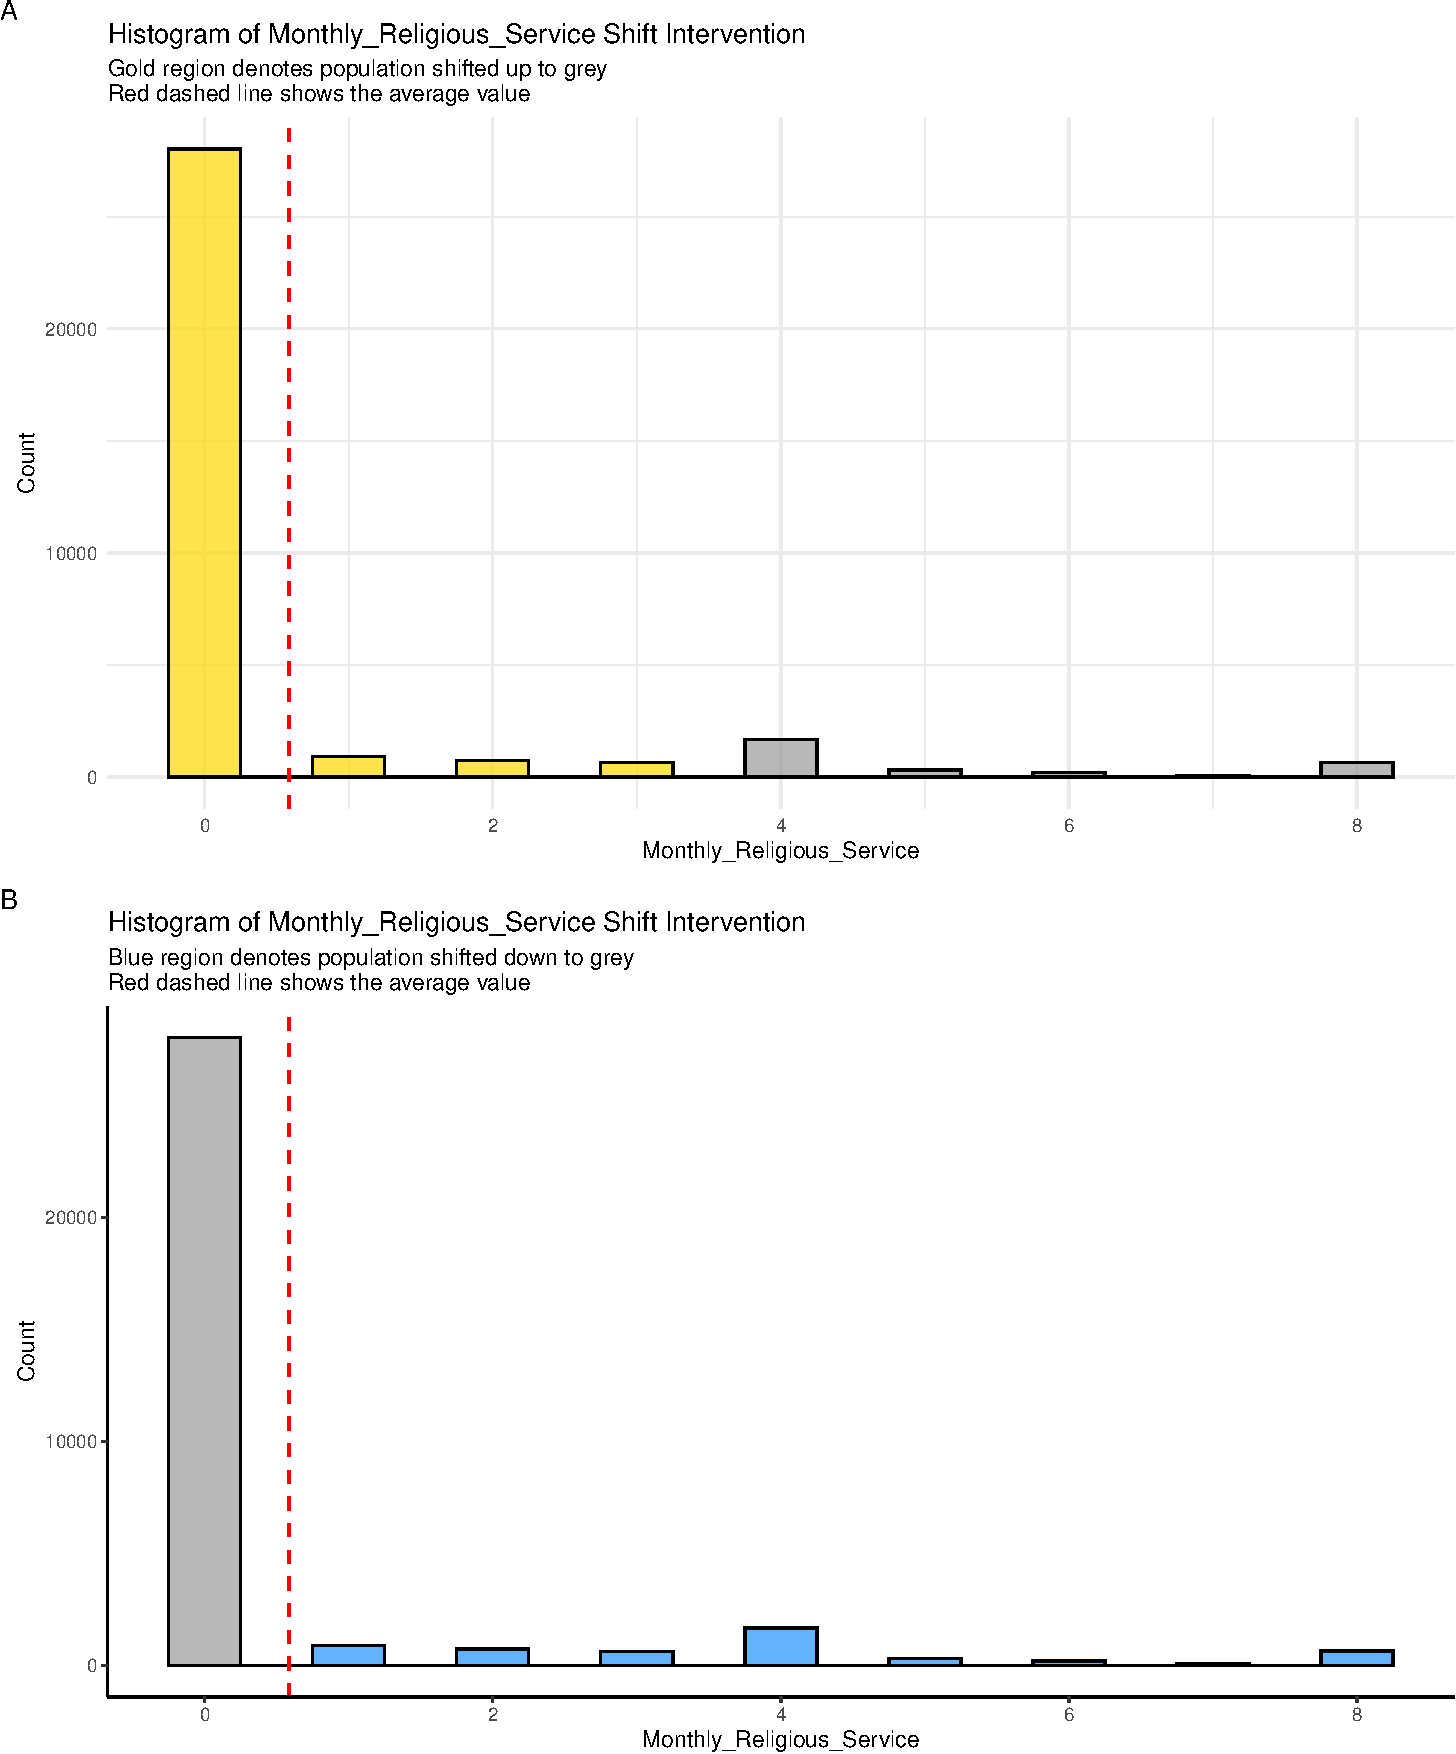
\includegraphics{test_files/figure-pdf/fig-hist-1.pdf}

}

\caption{\label{fig-hist}This figure shows a histogram of responses to
religious service frequency in the baseline + 1 wave. Responses above
eight were assigned to eight, and values were rounded to the nearest
whole number. The red dashed line shows the population average. (A)
Responses in the gold bars are shifted to four on the Regular Religious
Service intervention. All those responses in grey (four and above)
remain unchanged. (B) On the zero-intervention, responses in the blue
bars denote those shifted under the zero-intervention treatment.}

\end{figure}%

\newpage{}

\subsubsection{Evidence for Change in the Treatment
Variable}\label{evidence-for-change-in-the-treatment-variable}

Table~\ref{tbl-transition} clarifies the change in the treatment
variable from the baseline wave to the baseline + 1 wave across the
sample. Assessing change in a variable is essential for evaluating the
positivity assumption and recovering evidence for the incident exposure
effect of the treatment variable (\citeproc{ref-vanderweele2020}{Tyler
J. VanderWeele, Mathur, and Chen 2020};
\citeproc{ref-danaei2012}{Danaei, Tavakkoli, and Hernán 2012};
\citeproc{ref-hernan2024WHATIF}{Hernan and Robins 2024}). We find that
state 4 (weekly attendance) and state 0 present the highest overall.
However, movement between these states reveals they are not
deterministic. States 1, 2, 3, and 5 exhibit more frequent jumps in and
out of these states, suggesting lower stability and/or measurement
error.

\begin{longtable}[]{@{}
  >{\centering\arraybackslash}p{(\columnwidth - 18\tabcolsep) * \real{0.0978}}
  >{\centering\arraybackslash}p{(\columnwidth - 18\tabcolsep) * \real{0.1196}}
  >{\centering\arraybackslash}p{(\columnwidth - 18\tabcolsep) * \real{0.0978}}
  >{\centering\arraybackslash}p{(\columnwidth - 18\tabcolsep) * \real{0.0978}}
  >{\centering\arraybackslash}p{(\columnwidth - 18\tabcolsep) * \real{0.0978}}
  >{\centering\arraybackslash}p{(\columnwidth - 18\tabcolsep) * \real{0.0978}}
  >{\centering\arraybackslash}p{(\columnwidth - 18\tabcolsep) * \real{0.0978}}
  >{\centering\arraybackslash}p{(\columnwidth - 18\tabcolsep) * \real{0.0978}}
  >{\centering\arraybackslash}p{(\columnwidth - 18\tabcolsep) * \real{0.0978}}
  >{\centering\arraybackslash}p{(\columnwidth - 18\tabcolsep) * \real{0.0978}}@{}}

\caption{\label{tbl-transition}This transition matrix captures stability
and change in religious service between the baseline and treatment wave.
Each cell in the matrix represents the count of individuals
transitioning from one state to another. The rows correspond to the
state at baseline (From), and the columns correspond to the state at the
treatment wave (To). \textbf{Diagonal entries} (in \textbf{bold})
signify the number of individuals who remained in their initial state
across both waves. \textbf{Off-diagonal entries} signify the transitions
of individuals from their baseline state to a different state in the
treatment wave. A higher number on the diagonal relative to the
off-diagonal entries in the same row indicates greater stability in a
state. Conversely, higher off-diagonal numbers suggest more frequent
shifts in the sample from the baseline state to other states.}

\tabularnewline

\toprule\noalign{}
\begin{minipage}[b]{\linewidth}\centering
From
\end{minipage} & \begin{minipage}[b]{\linewidth}\centering
State 0
\end{minipage} & \begin{minipage}[b]{\linewidth}\centering
State 1
\end{minipage} & \begin{minipage}[b]{\linewidth}\centering
State 2
\end{minipage} & \begin{minipage}[b]{\linewidth}\centering
State 3
\end{minipage} & \begin{minipage}[b]{\linewidth}\centering
State 4
\end{minipage} & \begin{minipage}[b]{\linewidth}\centering
State 5
\end{minipage} & \begin{minipage}[b]{\linewidth}\centering
State 6
\end{minipage} & \begin{minipage}[b]{\linewidth}\centering
State 7
\end{minipage} & \begin{minipage}[b]{\linewidth}\centering
State 8
\end{minipage} \\
\midrule\noalign{}
\endhead
\bottomrule\noalign{}
\endlastfoot
State 0 & \textbf{26762} & 405 & 174 & 71 & 126 & 26 & 13 & 8 & 68 \\
State 1 & 647 & \textbf{235} & 85 & 44 & 46 & 5 & 2 & 3 & 10 \\
State 2 & 236 & 105 & \textbf{188} & 104 & 96 & 12 & 13 & 2 & 21 \\
State 3 & 112 & 54 & 110 & \textbf{164} & 173 & 18 & 8 & 4 & 15 \\
State 4 & 150 & 71 & 127 & 205 & \textbf{881} & 124 & 64 & 16 & 91 \\
State 5 & 24 & 7 & 17 & 17 & 145 & \textbf{61} & 25 & 7 & 33 \\
State 6 & 14 & 5 & 13 & 17 & 84 & 22 & \textbf{29} & 5 & 37 \\
State 7 & 9 & 0 & 6 & 3 & 16 & 6 & 9 & \textbf{6} & 19 \\
State 8 & 74 & 14 & 17 & 14 & 105 & 34 & 42 & 17 & \textbf{351} \\

\end{longtable}

\newpage{}

\subsection{Results}\label{results}

\subsubsection{Study 1: Causal Effects of Regular Church Attendance on
Self-Reported Volunteering and Self-Reported Volunteering and
Donations}\label{study-1-causal-effects-of-regular-church-attendance-on-self-reported-volunteering-and-self-reported-volunteering-and-donations}

\paragraph{Regular Religious Service vs.~Zero Treatment Contrast for
Donations and
Volunteering}\label{regular-religious-service-vs.-zero-treatment-contrast-for-donations-and-volunteering}

Results for the treatment contrasts between Regular Religious Service
and Zero Religious Service, focusing on self-reported volunteering and
charitable donations, are displayed in Figure~\ref{fig-1_1} \emph{A} and
Table~\ref{tbl-1_1}. These results are measured on the difference scale.

\begin{longtable}[]{@{}lrrrrr@{}}

\caption{\label{tbl-1_1}This table reports the results of model
estimates for the causal effects of a universal gain of weekly religious
service vs.~a universal loss of weekly religious service on reported
charitable behaviours at the end of the study. Contrasts are expressed
in standard deviation units.}

\tabularnewline

\toprule\noalign{}
& E{[}Y(1){]}-E{[}Y(0){]} & 2.5 \% & 97.5 \% & E\_Value &
E\_Val\_bound \\
\midrule\noalign{}
\endhead
\bottomrule\noalign{}
\endlastfoot
donations & 0.132 & 0.102 & 0.161 & 1.507 & 1.426 \\
hours volunteer & 0.123 & 0.090 & 0.156 & 1.482 & 1.389 \\

\end{longtable}

For `donations', the effect estimate is 0.132 {[}0.102, 0.161{]}. The
E-value for this estimate is 1.507, with a lower bound of 1.426. At this
lower bound, unmeasured confounders would need a minimum association
strength with both the intervention sequence and outcome of 1.426 to
negate the observed effect. Weaker associations would not overturn it.
We infer \textbf{evidence for causality}. On the data scale, this
intervention represents a difference of \textbf{NZD 656.58 per adult per
year} in charitable giving compared with the zero attendance
intervention.

The effect estimate for `hours volunteer' is 0.123 {[}0.09, 0.156{]}.
The E-value for this estimate is 1.482, with a lower bound of 1.389. We
infer \textbf{evidence for causality}. On the data scale, this
intervention represents a difference of \textbf{NZD 30.21 minutes} per
adult per week in volunteering compared with the zero attendance
intervention.

\paragraph{Regular Religious Service vs.~Status Quo Treatment Contrast
for Donations and
Volunteering}\label{regular-religious-service-vs.-status-quo-treatment-contrast-for-donations-and-volunteering}

Figure~\ref{fig-1_1} \emph{B} and Table~\ref{tbl-1_2} present results
for the treatment contrasts between Regular Religious Service and Status
Quo, focusing on self-reported volunteering and charitable donations.
These results are measured on the difference scale.

\begin{longtable}[]{@{}lrrrrr@{}}

\caption{\label{tbl-1_2}This table reports results of model estimates
for the causal effects of a universal gain of weekly religious service
vs.~the status quo on reported charitable behaviours at the end of the
study. Contrasts are expressed in standard deviation units.}

\tabularnewline

\toprule\noalign{}
& E{[}Y(1){]}-E{[}Y(0){]} & 2.5 \% & 97.5 \% & E\_Value &
E\_Val\_bound \\
\midrule\noalign{}
\endhead
\bottomrule\noalign{}
\endlastfoot
donations & 0.121 & 0.102 & 0.140 & 1.477 & 1.422 \\
hours volunteer & 0.095 & 0.066 & 0.123 & 1.404 & 1.317 \\

\end{longtable}

For `donations', the effect estimate is 0.121 {[}0.102, 0.14{]}. The
E-value for this estimate is 1.477, with a lower bound of 1.422. At this
lower bound, unmeasured confounders would need a minimum association
strength with both the intervention sequence and outcome of 1.422 to
negate the observed effect. Weaker confounding would not overturn it. We
infer \textbf{evidence for causality}. On the data scale, this
intervention represents an increase of \textbf{NZD 601.87 per adult per
year} in expected charitable giving over the status quo.

For `hours volunteer', the effect estimate is 0.095 {[}0.066, 0.123{]}.
The E-value for this estimate is 1.404, with a lower bound of 1.317. At
this lower bound, unmeasured confounders would need a minimum
association strength with both the intervention sequence and outcome of
1.317 to negate the observed effect. Weaker confounding would not
overturn it. We infer \textbf{evidence for causality}. On the data
scale, this intervention represents an increase of \textbf{23.33 minutes
} per adult per week in hours volunteering over the status quo.

\paragraph{Zero Religious Service vs.~The Status Quo Treatment Contrast
for Donations and
Volunteering}\label{zero-religious-service-vs.-the-status-quo-treatment-contrast-for-donations-and-volunteering}

Figure~\ref{fig-1_1} \emph{C} and Table~\ref{tbl-1_3} present results
for the treatment contrasts between Zero Religious Service and Status
Quo, focusing on self-reported volunteering and charitable donations.
These results are measured on the difference scale.

\begin{longtable}[]{@{}
  >{\raggedright\arraybackslash}p{(\columnwidth - 10\tabcolsep) * \real{0.2424}}
  >{\raggedleft\arraybackslash}p{(\columnwidth - 10\tabcolsep) * \real{0.2424}}
  >{\raggedleft\arraybackslash}p{(\columnwidth - 10\tabcolsep) * \real{0.1061}}
  >{\raggedleft\arraybackslash}p{(\columnwidth - 10\tabcolsep) * \real{0.1061}}
  >{\raggedleft\arraybackslash}p{(\columnwidth - 10\tabcolsep) * \real{0.1212}}
  >{\raggedleft\arraybackslash}p{(\columnwidth - 10\tabcolsep) * \real{0.1818}}@{}}

\caption{\label{tbl-1_3}This table reports the results of model
estimates for the causal effects of a universal loss of weekly religious
service vs.~the status quo on reported charitable behaviours at the end
of the study. Contrasts are expressed in standard deviation units.}

\tabularnewline

\toprule\noalign{}
\begin{minipage}[b]{\linewidth}\raggedright
\end{minipage} & \begin{minipage}[b]{\linewidth}\raggedleft
E{[}Y(1){]}-E{[}Y(0){]}
\end{minipage} & \begin{minipage}[b]{\linewidth}\raggedleft
2.5 \%
\end{minipage} & \begin{minipage}[b]{\linewidth}\raggedleft
97.5 \%
\end{minipage} & \begin{minipage}[b]{\linewidth}\raggedleft
E\_Value
\end{minipage} & \begin{minipage}[b]{\linewidth}\raggedleft
E\_Val\_bound
\end{minipage} \\
\midrule\noalign{}
\endhead
\bottomrule\noalign{}
\endlastfoot
donations & -0.011 & -0.029 & 0.008 & 1.111 & 1.000 \\
hours volunteer & -0.028 & -0.042 & -0.014 & 1.189 & 1.128 \\

\end{longtable}

For `donations', the effect estimate is -0.011 {[}-0.029, 0.008{]}. The
E-value for this estimate is 1.111, with a lower bound of 1. At this
lower bound, unmeasured confounders would need a minimum association
strength with both the intervention sequence and outcome of 1 to negate
the observed effect. Weaker confounding would not overturn it. We infer
that \textbf{the evidence for causality is not reliable}. On the data
scale, this intervention represents a difference of NZD -54.72 per adult
per year in charitable giving compared to the status quo. Still, again,
this effect is not reliable.

The effect estimate for `hours volunteer' is -0.028 {[}-0.042,
-0.014{]}. The E-value for this estimate is 1.189, with a lower bound of
1.128. At this lower bound, unmeasured confounders would need a minimum
association strength with both the intervention sequence and outcome of
1.128 to negate the observed effect. Again, weaker confounding would not
overturn it. We infer \textbf{evidence for causality}. \textbf{On the
data scale, this intervention represents a difference of -6.88 in
volunteering minutes compared with the status quo.}

\begin{figure}

\centering{

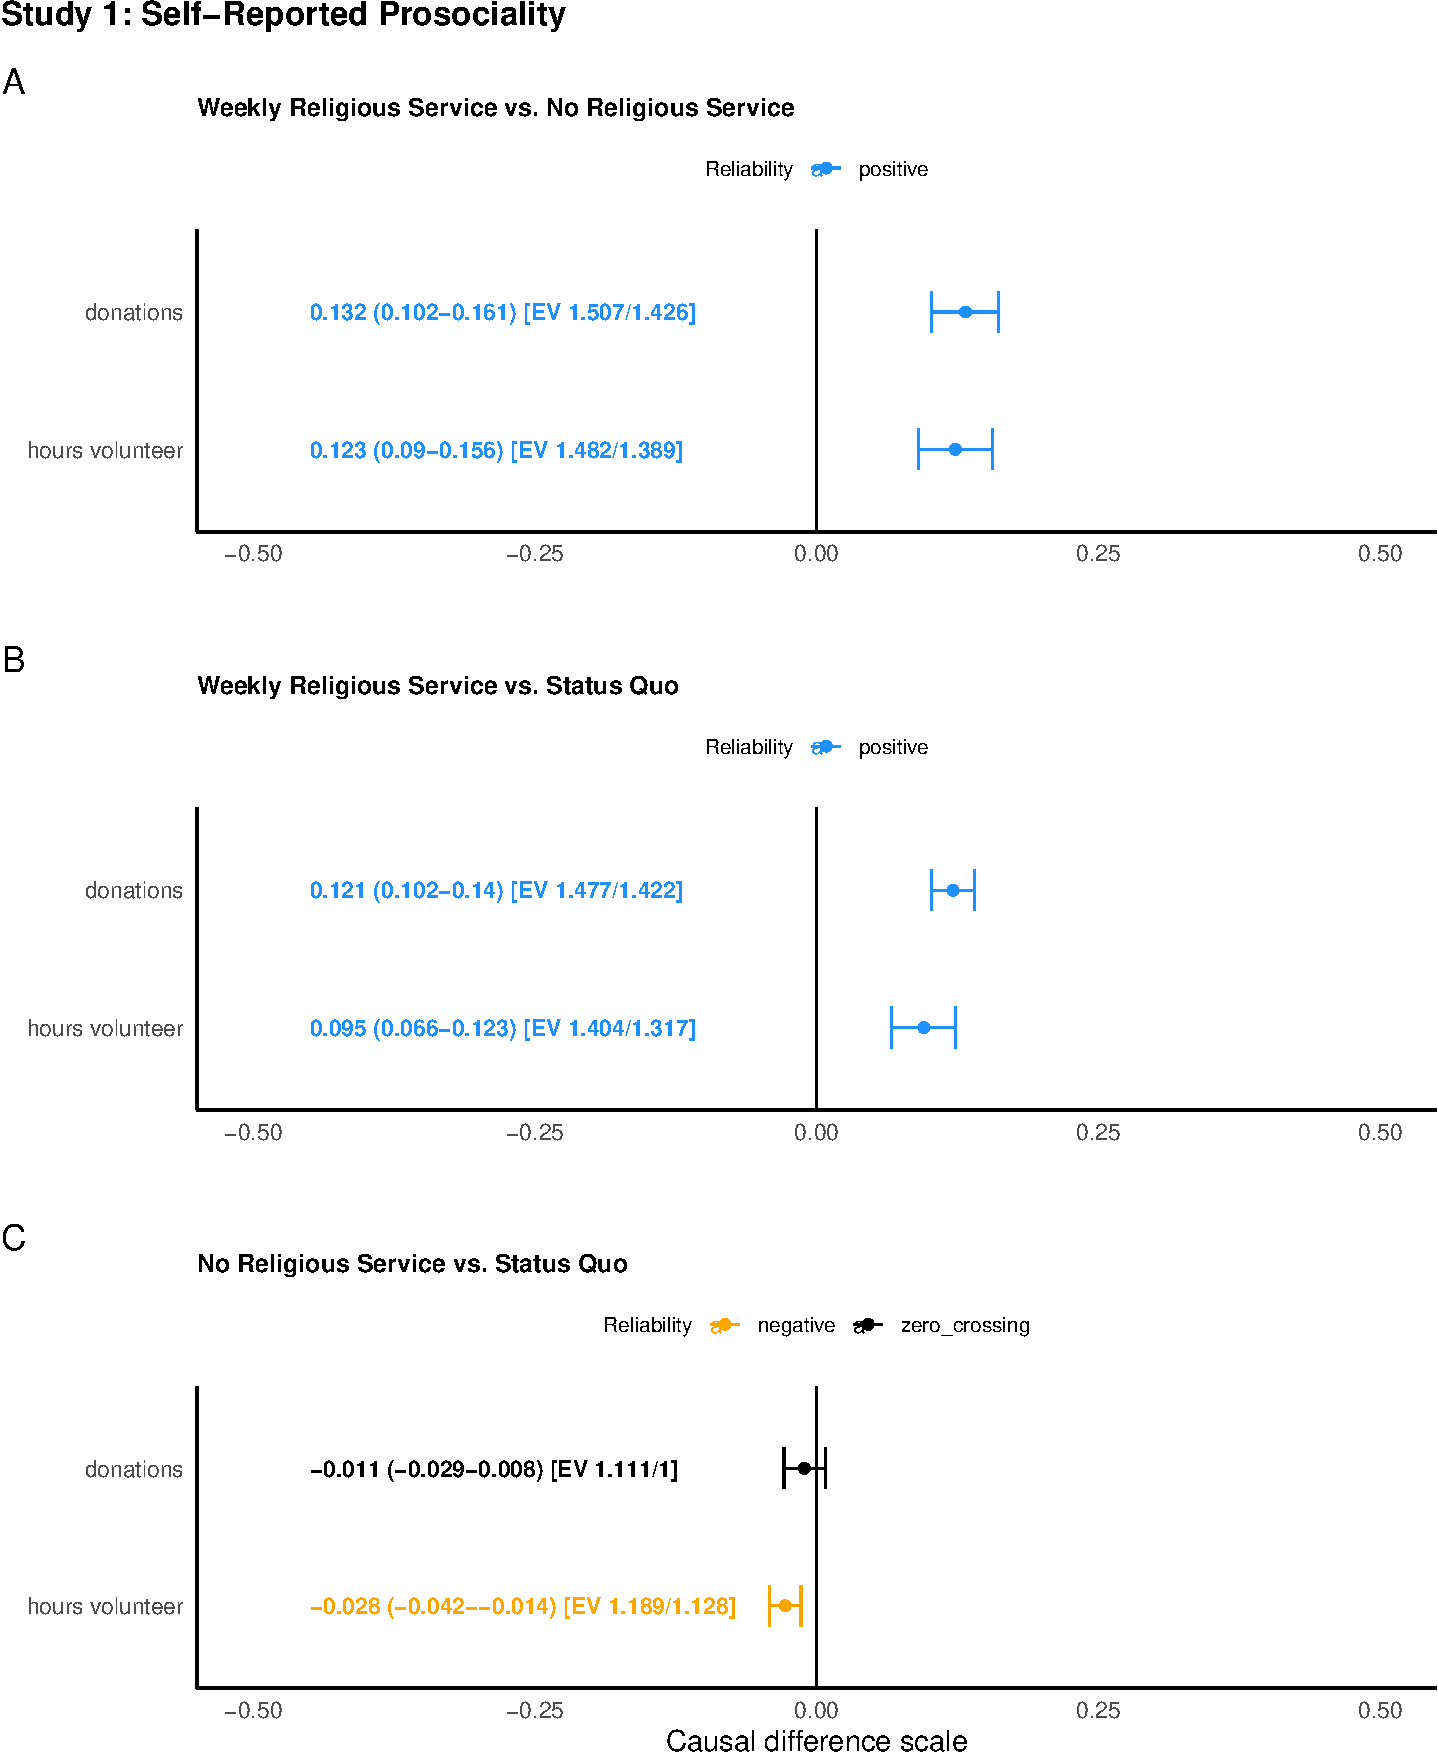
\includegraphics{test_files/figure-pdf/fig-1_1-1.pdf}

}

\caption{\label{fig-1_1}This figure graphs the results of model
estimates for the causal effects of the three causal contrasts of
interest on reported charitable behaviours at the study's end. The
causal contrasts are: (A) Regular vs.~Zero Religious Service, (B)
Regular Religious Service vs.~Status Quo, and (C) Zero Religious Service
vs.~Status Quo. Contrasts are expressed in standard deviation units.}

\end{figure}%

\newpage{}

\subsubsection{Study 2: Causal Effects of Regular Church Attendance on
Support Received From Others --
Time}\label{study-2-causal-effects-of-regular-church-attendance-on-support-received-from-others-time}

\paragraph{Regular vs.~Zero Causal Treatment Contrast for Time Received
From
Others}\label{regular-vs.-zero-causal-treatment-contrast-for-time-received-from-others}

Figure~\ref{fig-study2} \emph{A} and Table~\ref{tbl-study2A} present
results for the treatment contrasts between Regular Religious Service
and Zero, focusing on voluntary help received from others during the
past week (yes/no). These results are measured on the risk ratio scale.

\begin{longtable}[]{@{}
  >{\raggedright\arraybackslash}p{(\columnwidth - 10\tabcolsep) * \real{0.3000}}
  >{\raggedleft\arraybackslash}p{(\columnwidth - 10\tabcolsep) * \real{0.2286}}
  >{\raggedleft\arraybackslash}p{(\columnwidth - 10\tabcolsep) * \real{0.0857}}
  >{\raggedleft\arraybackslash}p{(\columnwidth - 10\tabcolsep) * \real{0.1000}}
  >{\raggedleft\arraybackslash}p{(\columnwidth - 10\tabcolsep) * \real{0.1143}}
  >{\raggedleft\arraybackslash}p{(\columnwidth - 10\tabcolsep) * \real{0.1714}}@{}}

\caption{\label{tbl-study2A}This table reports the results of model
estimates for the causal effects of a universal gain of weekly religious
service vs.~a universal loss of weekly religious service on voluntary
help received from others during the past week (yes/no) at the end of
the study. Contrasts are expressed on the risk ratio scale.}

\tabularnewline

\toprule\noalign{}
\begin{minipage}[b]{\linewidth}\raggedright
\end{minipage} & \begin{minipage}[b]{\linewidth}\raggedleft
E{[}Y(1){]}/E{[}Y(0){]}
\end{minipage} & \begin{minipage}[b]{\linewidth}\raggedleft
2.5 \%
\end{minipage} & \begin{minipage}[b]{\linewidth}\raggedleft
97.5 \%
\end{minipage} & \begin{minipage}[b]{\linewidth}\raggedleft
E\_Value
\end{minipage} & \begin{minipage}[b]{\linewidth}\raggedleft
E\_Val\_bound
\end{minipage} \\
\midrule\noalign{}
\endhead
\bottomrule\noalign{}
\endlastfoot
family gives time & 0.950 & 0.901 & 1.003 & 1.288 & 1.000 \\
friends give time & 1.187 & 1.108 & 1.271 & 1.658 & 1.454 \\
community gives time & 1.378 & 1.231 & 1.541 & 2.100 & 1.764 \\

\end{longtable}

For `community gives time', the effect estimate is 1.378 {[}1.231,
1.541{]}. The E-value for this estimate is 2.1, with a lower bound of
1.764. At this lower bound, unmeasured confounders would need a minimum
association strength with both the intervention sequence and outcome of
1.764 to negate the observed effect. Weaker confounding would not
overturn it. We infer \textbf{evidence for causality}.

For `friends give time', the effect estimate is 1.187 {[}1.108,
1.271{]}. The E-value for this estimate is 1.658, with a lower bound of
1.454. At this lower bound, unmeasured confounders would need a minimum
association strength with both the intervention sequence and outcome of
1.454 to negate the observed effect. Weaker confounding would not
overturn it. We infer \textbf{evidence for causality}.

For `family gives time', the effect estimate is 0.95 {[}0.901, 1.003{]}.
The E-value for this estimate is 1.288, with a lower bound of 1. At this
lower bound, unmeasured confounders would need a minimum association
strength with both the intervention sequence and outcome of 1 to negate
the observed effect. Weaker confounding would not overturn it. We infer
\textbf{that evidence for causality is not reliable}.

\paragraph{Regular Religious Service vs.~Status Quo Treatment Contrast
for Time Received From
Others}\label{regular-religious-service-vs.-status-quo-treatment-contrast-for-time-received-from-others}

Figure~\ref{fig-study2}\emph{B} and Table~\ref{tbl-2-2} present results
for the treatment contrasts between Regular Religious Service and Status
Quo, focusing on voluntary help received from others during the past
week (yes/no). These results are measured on the risk ratio scale.

\begin{longtable}[]{@{}
  >{\raggedright\arraybackslash}p{(\columnwidth - 10\tabcolsep) * \real{0.3000}}
  >{\raggedleft\arraybackslash}p{(\columnwidth - 10\tabcolsep) * \real{0.2286}}
  >{\raggedleft\arraybackslash}p{(\columnwidth - 10\tabcolsep) * \real{0.0857}}
  >{\raggedleft\arraybackslash}p{(\columnwidth - 10\tabcolsep) * \real{0.1000}}
  >{\raggedleft\arraybackslash}p{(\columnwidth - 10\tabcolsep) * \real{0.1143}}
  >{\raggedleft\arraybackslash}p{(\columnwidth - 10\tabcolsep) * \real{0.1714}}@{}}

\caption{\label{tbl-2-2}This table reports the results of model
estimates for the causal effects of a universal gain of weekly religious
service vs.~the status quo on voluntary help received from others during
the past week (yes/no) at the end of the study. Contrasts are expressed
on the risk ratio scale.}

\tabularnewline

\toprule\noalign{}
\begin{minipage}[b]{\linewidth}\raggedright
\end{minipage} & \begin{minipage}[b]{\linewidth}\raggedleft
E{[}Y(1){]}/E{[}Y(0){]}
\end{minipage} & \begin{minipage}[b]{\linewidth}\raggedleft
2.5 \%
\end{minipage} & \begin{minipage}[b]{\linewidth}\raggedleft
97.5 \%
\end{minipage} & \begin{minipage}[b]{\linewidth}\raggedleft
E\_Value
\end{minipage} & \begin{minipage}[b]{\linewidth}\raggedleft
E\_Val\_bound
\end{minipage} \\
\midrule\noalign{}
\endhead
\bottomrule\noalign{}
\endlastfoot
family gives time & 0.958 & 0.913 & 1.006 & 1.258 & 1.000 \\
friends give time & 1.128 & 1.061 & 1.199 & 1.508 & 1.315 \\
community gives time & 1.289 & 1.174 & 1.415 & 1.899 & 1.626 \\

\end{longtable}

For `community gives time', the effect estimate is 1.289 {[}1.174,
1.415{]}. The E-value for this estimate is 1.899, with a lower bound of
1.626. At this lower bound, unmeasured confounders would need a minimum
association strength with both the intervention sequence and outcome of
1.626 to negate the observed effect. Weaker confounding would not
overturn it. We infer \textbf{evidence for causality}.

For `friends give time', the effect estimate is 1.128 {[}1.061,
1.199{]}. The E-value for this estimate is 1.508, with a lower bound of
1.315. At this lower bound, unmeasured confounders would need a minimum
association strength with both the intervention sequence and outcome of
1.315 to negate the observed effect. Weaker confounding would not
overturn it. We infer \textbf{evidence for causality}.

For `family gives time', the effect estimate is 0.958 {[}0.913,
1.006{]}. The E-value for this estimate is 1.258, with a lower bound of
1. At this lower bound, unmeasured confounders would need a minimum
association strength with both the intervention sequence and outcome of
1 to negate the observed effect. Weaker confounding would not overturn
it. We infer \textbf{that evidence for causality is not reliable}.

\paragraph{Zero Religious Service vs.~Status Quo Treatment Contrast for
Time Received From
Others}\label{zero-religious-service-vs.-status-quo-treatment-contrast-for-time-received-from-others}

Figure~\ref{fig-study2} \emph{C} and Table~\ref{tbl-2_3} present results
for the treatment contrasts between Zero Religious Service and Status
Quo, focusing on voluntary help received from others during the past
week (yes/no). These results are measured on the risk ratio scale.

\begin{longtable}[]{@{}
  >{\raggedright\arraybackslash}p{(\columnwidth - 10\tabcolsep) * \real{0.3000}}
  >{\raggedleft\arraybackslash}p{(\columnwidth - 10\tabcolsep) * \real{0.2286}}
  >{\raggedleft\arraybackslash}p{(\columnwidth - 10\tabcolsep) * \real{0.0857}}
  >{\raggedleft\arraybackslash}p{(\columnwidth - 10\tabcolsep) * \real{0.1000}}
  >{\raggedleft\arraybackslash}p{(\columnwidth - 10\tabcolsep) * \real{0.1143}}
  >{\raggedleft\arraybackslash}p{(\columnwidth - 10\tabcolsep) * \real{0.1714}}@{}}

\caption{\label{tbl-2_3}This table reports results of model estimates
for the causal effects of a universal loss of weekly religious service
vs.~the status quo on voluntary help received from others during the
past week (yes/no) at the end of the study. Contrasts are expressed on
the risk ratio scale.}

\tabularnewline

\toprule\noalign{}
\begin{minipage}[b]{\linewidth}\raggedright
\end{minipage} & \begin{minipage}[b]{\linewidth}\raggedleft
E{[}Y(1){]}/E{[}Y(0){]}
\end{minipage} & \begin{minipage}[b]{\linewidth}\raggedleft
2.5 \%
\end{minipage} & \begin{minipage}[b]{\linewidth}\raggedleft
97.5 \%
\end{minipage} & \begin{minipage}[b]{\linewidth}\raggedleft
E\_Value
\end{minipage} & \begin{minipage}[b]{\linewidth}\raggedleft
E\_Val\_bound
\end{minipage} \\
\midrule\noalign{}
\endhead
\bottomrule\noalign{}
\endlastfoot
family gives time & 1.008 & 0.991 & 1.026 & 1.098 & 1.000 \\
friends give time & 0.950 & 0.928 & 0.973 & 1.288 & 1.197 \\
community gives time & 0.936 & 0.889 & 0.985 & 1.339 & 1.140 \\

\end{longtable}

For `family gives time', the effect estimate is 1.008 {[}0.991,
1.026{]}. The E-value for this estimate is 1.098, with a lower bound of
1. At this lower bound, unmeasured confounders would need a minimum
association strength with both the intervention sequence and outcome of
1 to negate the observed effect. Weaker confounding would not overturn
it. We infer \textbf{that evidence for causality is not reliable}.

For `friends give time', the effect estimate is 0.95 {[}0.928, 0.973{]}.
The E-value for this estimate is 1.288, with a lower bound of 1.197. At
this lower bound, unmeasured confounders would need a minimum
association strength with both the intervention sequence and outcome of
1.197 to negate the observed effect. Weaker confounding would not
overturn it. We infer \textbf{evidence for causality}.

For `community gives time', the effect estimate is 0.936 {[}0.889,
0.985{]}. The E-value for this estimate is 1.339, with a lower bound of
1.14. At this lower bound, unmeasured confounders would need a minimum
association strength with both the intervention sequence and outcome of
1.14 to negate the observed effect. Weaker confounding would not
overturn it. We infer \textbf{evidence for causality}.

\begin{figure}

\centering{

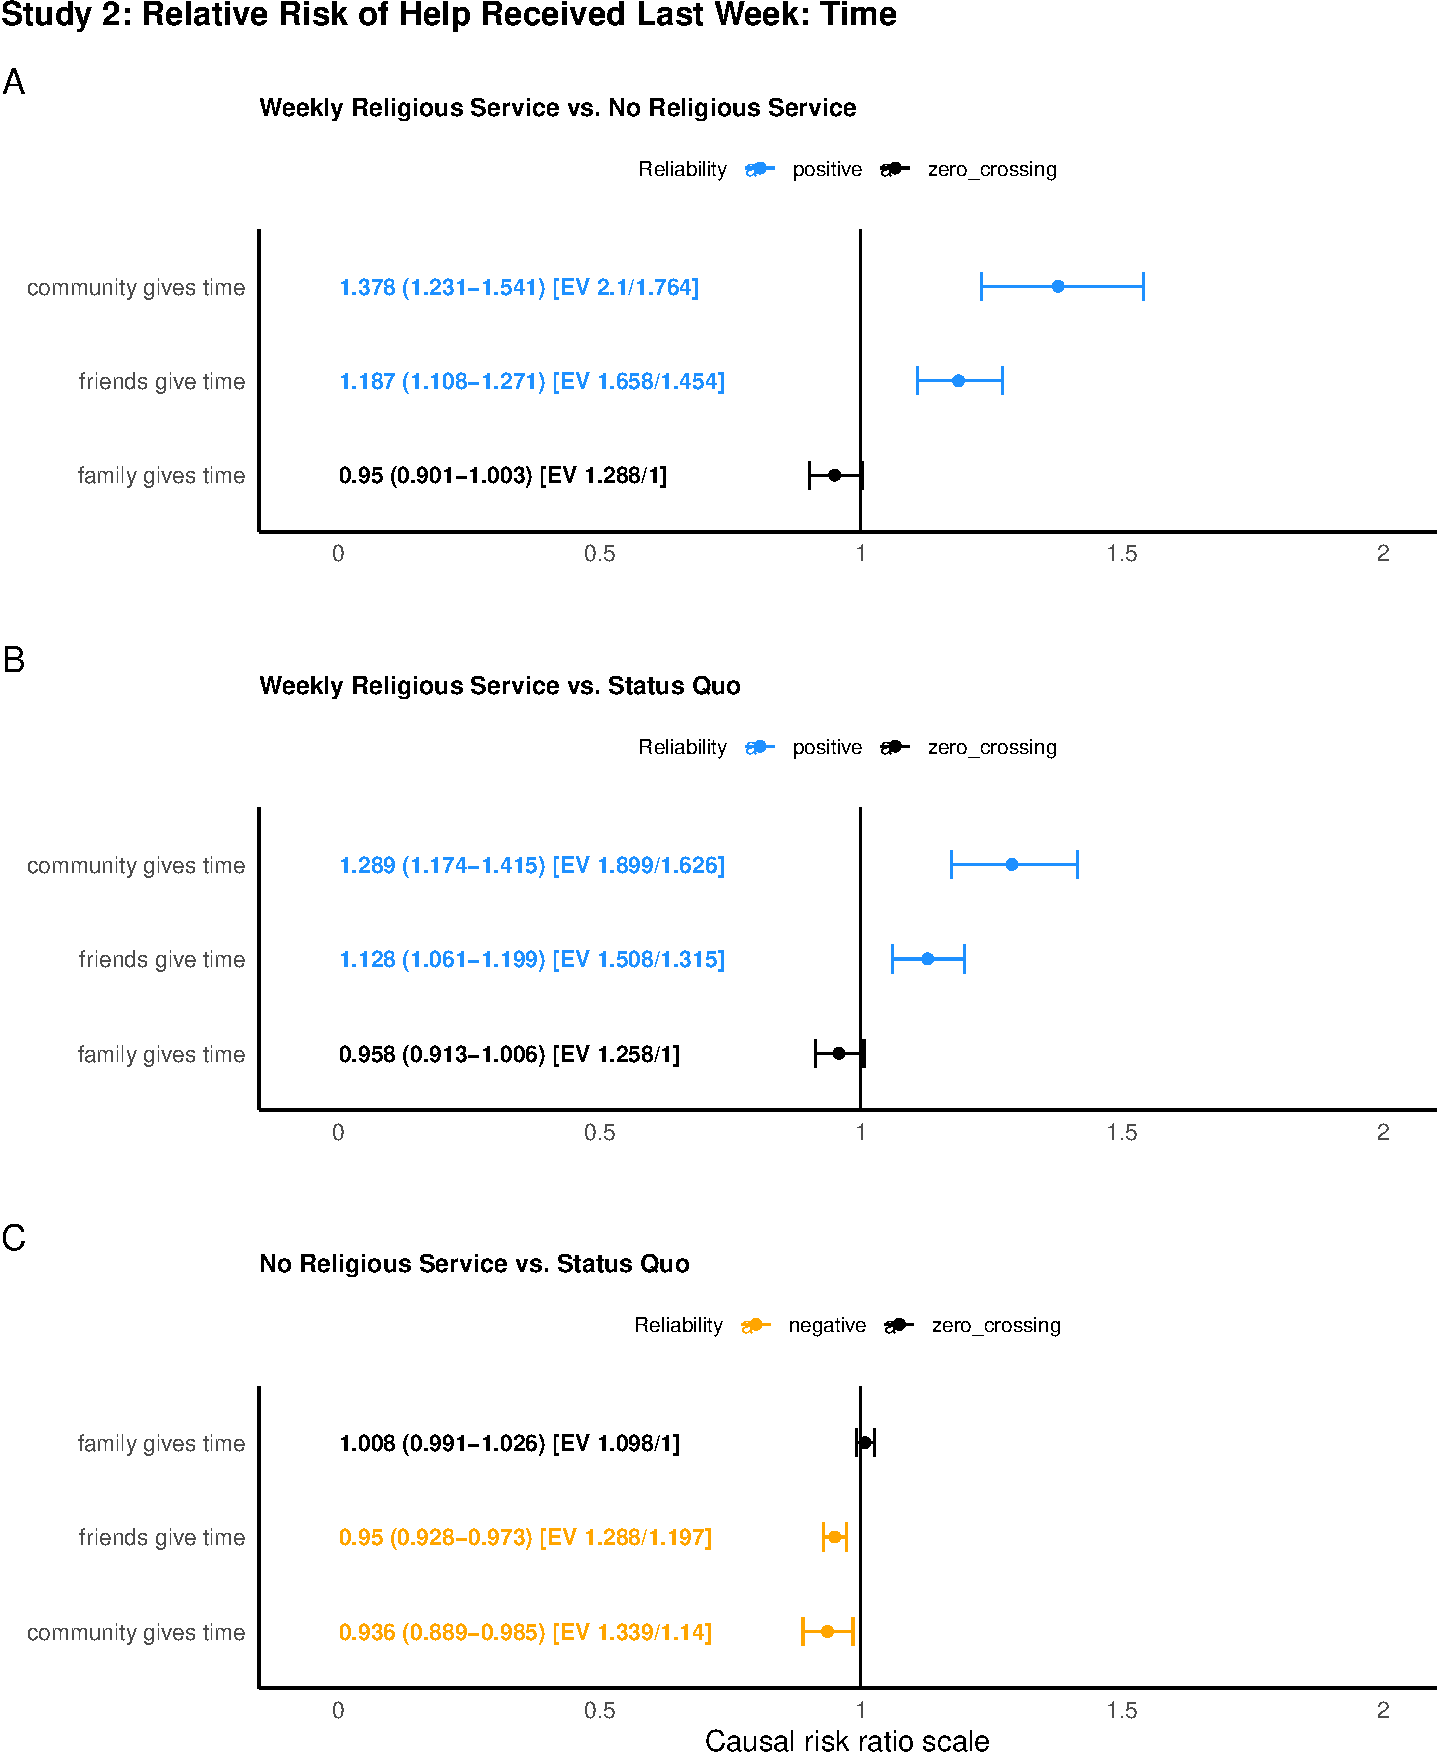
\includegraphics{test_files/figure-pdf/fig-study2-1.pdf}

}

\caption{\label{fig-study2}This figure reports the results of model
estimates for the three causal contrasts of interest on help received
from others during the past week (yes/no). The causal contrasts are (A)
Regular vs.~Zero Religious Service, (B) Regular Religious Service
vs.~Status Quo, and (C) Zero Religious Service vs.~Status Quo. Contrasts
are expressed on the risk ratio scale.}

\end{figure}%

\newpage{}

\subsubsection{Study 3: Causal Effects of Regular Church Attendance on
Support Received From Others --
Money}\label{study-3-causal-effects-of-regular-church-attendance-on-support-received-from-others-money}

\paragraph{Regular vs.~Zero Causal Contrast on Money Received From
Others}\label{regular-vs.-zero-causal-contrast-on-money-received-from-others}

Figure~\ref{fig-study_3} \emph{A} and Table~\ref{tbl-3_1} present
results for the treatment contrasts between Regular Religious Service
and Zero, focusing on money received from others during the past week
(yes/no). These results are measured on the risk ratio scale.

\begin{longtable}[]{@{}
  >{\raggedright\arraybackslash}p{(\columnwidth - 10\tabcolsep) * \real{0.3099}}
  >{\raggedleft\arraybackslash}p{(\columnwidth - 10\tabcolsep) * \real{0.2254}}
  >{\raggedleft\arraybackslash}p{(\columnwidth - 10\tabcolsep) * \real{0.0845}}
  >{\raggedleft\arraybackslash}p{(\columnwidth - 10\tabcolsep) * \real{0.0986}}
  >{\raggedleft\arraybackslash}p{(\columnwidth - 10\tabcolsep) * \real{0.1127}}
  >{\raggedleft\arraybackslash}p{(\columnwidth - 10\tabcolsep) * \real{0.1690}}@{}}

\caption{\label{tbl-3_1}This table reports the results of model
estimates for the causal effects of a universal gain of weekly religious
service vs.~a universal loss of weekly religious service on financial
help received from others during the past week (yes/no) at the end of
the study. Contrasts are expressed on the risk ratio scale.}

\tabularnewline

\toprule\noalign{}
\begin{minipage}[b]{\linewidth}\raggedright
\end{minipage} & \begin{minipage}[b]{\linewidth}\raggedleft
E{[}Y(1){]}/E{[}Y(0){]}
\end{minipage} & \begin{minipage}[b]{\linewidth}\raggedleft
2.5 \%
\end{minipage} & \begin{minipage}[b]{\linewidth}\raggedleft
97.5 \%
\end{minipage} & \begin{minipage}[b]{\linewidth}\raggedleft
E\_Value
\end{minipage} & \begin{minipage}[b]{\linewidth}\raggedleft
E\_Val\_bound
\end{minipage} \\
\midrule\noalign{}
\endhead
\bottomrule\noalign{}
\endlastfoot
family gives money & 1.137 & 1.028 & 1.258 & 1.532 & 1.198 \\
friends give money & 1.137 & 0.964 & 1.342 & 1.532 & 1.000 \\
community gives money & 1.376 & 1.112 & 1.703 & 2.095 & 1.465 \\

\end{longtable}

For `community gives money', the effect estimate is 1.376 {[}1.112,
1.703{]}. The E-value for this estimate is 2.095, with a lower bound of
1.465. At this lower bound, unmeasured confounders would need a minimum
association strength with both the intervention sequence and outcome of
1.465 to negate the observed effect. Weaker confounding would not
overturn it. We infer \textbf{evidence for causality}.

For `family gives money', the effect estimate is 1.137 {[}1.028,
1.258{]}. The E-value for this estimate is 1.532, with a lower bound of
1.198. At this lower bound, unmeasured confounders would need a minimum
association strength with both the intervention sequence and outcome of
1.198 to negate the observed effect. Weaker confounding would not
overturn it. We infer \textbf{evidence for causality}.

For `friends give money', the effect estimate is 1.137 {[}0.964,
1.342{]}. The E-value for this estimate is 1.532, with a lower bound of
1. At this lower bound, unmeasured confounders would need a minimum
association strength with both the intervention sequence and outcome of
1 to negate the observed effect. Weaker confounding would not overturn
it. We infer \textbf{that evidence for causality is not reliable}.

\paragraph{Regular vs.~Status Quo Causal Contrast on Money Received From
Others}\label{regular-vs.-status-quo-causal-contrast-on-money-received-from-others}

Figure~\ref{fig-study_3} \emph{B} and Table~\ref{tbl-3_2} present
results for the treatment contrasts between Regular Religious Service
and Status Quo, focusing on money received from others during the past
week (yes/no). These results are measured on the risk ratio scale.

\begin{longtable}[]{@{}
  >{\raggedright\arraybackslash}p{(\columnwidth - 10\tabcolsep) * \real{0.3099}}
  >{\raggedleft\arraybackslash}p{(\columnwidth - 10\tabcolsep) * \real{0.2254}}
  >{\raggedleft\arraybackslash}p{(\columnwidth - 10\tabcolsep) * \real{0.0845}}
  >{\raggedleft\arraybackslash}p{(\columnwidth - 10\tabcolsep) * \real{0.0986}}
  >{\raggedleft\arraybackslash}p{(\columnwidth - 10\tabcolsep) * \real{0.1127}}
  >{\raggedleft\arraybackslash}p{(\columnwidth - 10\tabcolsep) * \real{0.1690}}@{}}

\caption{\label{tbl-3_2}This table reports the results of model
estimates for the causal effects of a universal gain of weekly religious
service vs.~the status quo on financial help received from others during
the past week (yes/no) at the end of the study. Contrasts are expressed
on the risk ratio scale.}

\tabularnewline

\toprule\noalign{}
\begin{minipage}[b]{\linewidth}\raggedright
\end{minipage} & \begin{minipage}[b]{\linewidth}\raggedleft
E{[}Y(1){]}/E{[}Y(0){]}
\end{minipage} & \begin{minipage}[b]{\linewidth}\raggedleft
2.5 \%
\end{minipage} & \begin{minipage}[b]{\linewidth}\raggedleft
97.5 \%
\end{minipage} & \begin{minipage}[b]{\linewidth}\raggedleft
E\_Value
\end{minipage} & \begin{minipage}[b]{\linewidth}\raggedleft
E\_Val\_bound
\end{minipage} \\
\midrule\noalign{}
\endhead
\bottomrule\noalign{}
\endlastfoot
family gives money & 1.130 & 1.037 & 1.232 & 1.513 & 1.233 \\
friends give money & 1.041 & 0.951 & 1.139 & 1.248 & 1.000 \\
community gives money & 1.254 & 1.098 & 1.432 & 1.818 & 1.426 \\

\end{longtable}

For `community gives money', the effect estimate is 1.254 {[}1.098,
1.432{]}. The E-value for this estimate is 1.818, with a lower bound of
1.426. At this lower bound, unmeasured confounders would need a minimum
association strength with both the intervention sequence and outcome of
1.426 to negate the observed effect. Weaker confounding would not
overturn it. We infer \textbf{evidence for causality}.

For `family gives money', the effect estimate is 1.13 {[}1.037,
1.232{]}. The E-value for this estimate is 1.513, with a lower bound of
1.233. At this lower bound, unmeasured confounders would need a minimum
association strength with both the intervention sequence and outcome of
1.233 to negate the observed effect. Weaker confounding would not
overturn it. We infer \textbf{evidence for causality}.

For `friends give money', the effect estimate is 1.041 {[}0.951,
1.139{]}. The E-value for this estimate is 1.248, with a lower bound of
1. At this lower bound, unmeasured confounders would need a minimum
association strength with both the intervention sequence and outcome of
1 to negate the observed effect. Weaker confounding would not overturn
it. We infer \textbf{that evidence for causality is not reliable}.

\paragraph{Zero vs.~Status Quo Causal Contrast on Money Received From
Others}\label{zero-vs.-status-quo-causal-contrast-on-money-received-from-others}

Figure~\ref{fig-study_3} \emph{C} and Table~\ref{tbl-3_3} present
results for the treatment contrasts between Zero Religious Service and
Status Quo, focusing on money received from others during the past week
(yes/no). These results are measured on the risk ratio scale.

\begin{longtable}[]{@{}
  >{\raggedright\arraybackslash}p{(\columnwidth - 10\tabcolsep) * \real{0.3099}}
  >{\raggedleft\arraybackslash}p{(\columnwidth - 10\tabcolsep) * \real{0.2254}}
  >{\raggedleft\arraybackslash}p{(\columnwidth - 10\tabcolsep) * \real{0.0845}}
  >{\raggedleft\arraybackslash}p{(\columnwidth - 10\tabcolsep) * \real{0.0986}}
  >{\raggedleft\arraybackslash}p{(\columnwidth - 10\tabcolsep) * \real{0.1127}}
  >{\raggedleft\arraybackslash}p{(\columnwidth - 10\tabcolsep) * \real{0.1690}}@{}}

\caption{\label{tbl-3_3}Table reports results of model estimates for the
causal effects of a universal loss of weekly religious service vs.~the
status quo on financial help received from others during the past week
(yes/no) at the end of study. Contrasts are expressed on the risk ratio
scale.}

\tabularnewline

\toprule\noalign{}
\begin{minipage}[b]{\linewidth}\raggedright
\end{minipage} & \begin{minipage}[b]{\linewidth}\raggedleft
E{[}Y(1){]}/E{[}Y(0){]}
\end{minipage} & \begin{minipage}[b]{\linewidth}\raggedleft
2.5 \%
\end{minipage} & \begin{minipage}[b]{\linewidth}\raggedleft
97.5 \%
\end{minipage} & \begin{minipage}[b]{\linewidth}\raggedleft
E\_Value
\end{minipage} & \begin{minipage}[b]{\linewidth}\raggedleft
E\_Val\_bound
\end{minipage} \\
\midrule\noalign{}
\endhead
\bottomrule\noalign{}
\endlastfoot
family gives money & 0.993 & 0.953 & 1.035 & 1.091 & 1 \\
friends gives money & 0.915 & 0.809 & 1.036 & 1.412 & 1 \\
community gives money & 0.911 & 0.796 & 1.042 & 1.425 & 1 \\

\end{longtable}

For `family gives money', the effect estimate on the risk ratio scale is
0.993 {[}0.953, 1.035{]}. The E-value for this estimate is 1.091, with a
lower bound of 1. At this lower bound, unmeasured confounders would need
a minimum association strength with both the intervention sequence and
outcome of 1 to negate the observed effect. Weaker confounding would not
overturn it. We infer \textbf{that evidence for causality is not
reliable}.

For `friends give money', the effect estimate on the risk ratio scale is
0.915 {[}0.809, 1.036{]}. The E-value for this estimate is 1.412, with a
lower bound of 1. At this lower bound, unmeasured confounders would need
a minimum association strength with both the intervention sequence and
outcome of 1 to negate the observed effect. Weaker confounding would not
overturn it. We infer \textbf{that evidence for causality is not
reliable}.

For `community gives money', the effect estimate on the risk ratio scale
is 0.911 {[}0.796, 1.042{]}. The E-value for this estimate is 1.425,
with a lower bound of 1. At this lower bound, unmeasured confounders
would need a minimum association strength with both the intervention
sequence and outcome of 1 to negate the observed effect. Weaker
confounding would not overturn it. We infer \textbf{that evidence for
causality is not reliable}.

\begin{figure}

\centering{

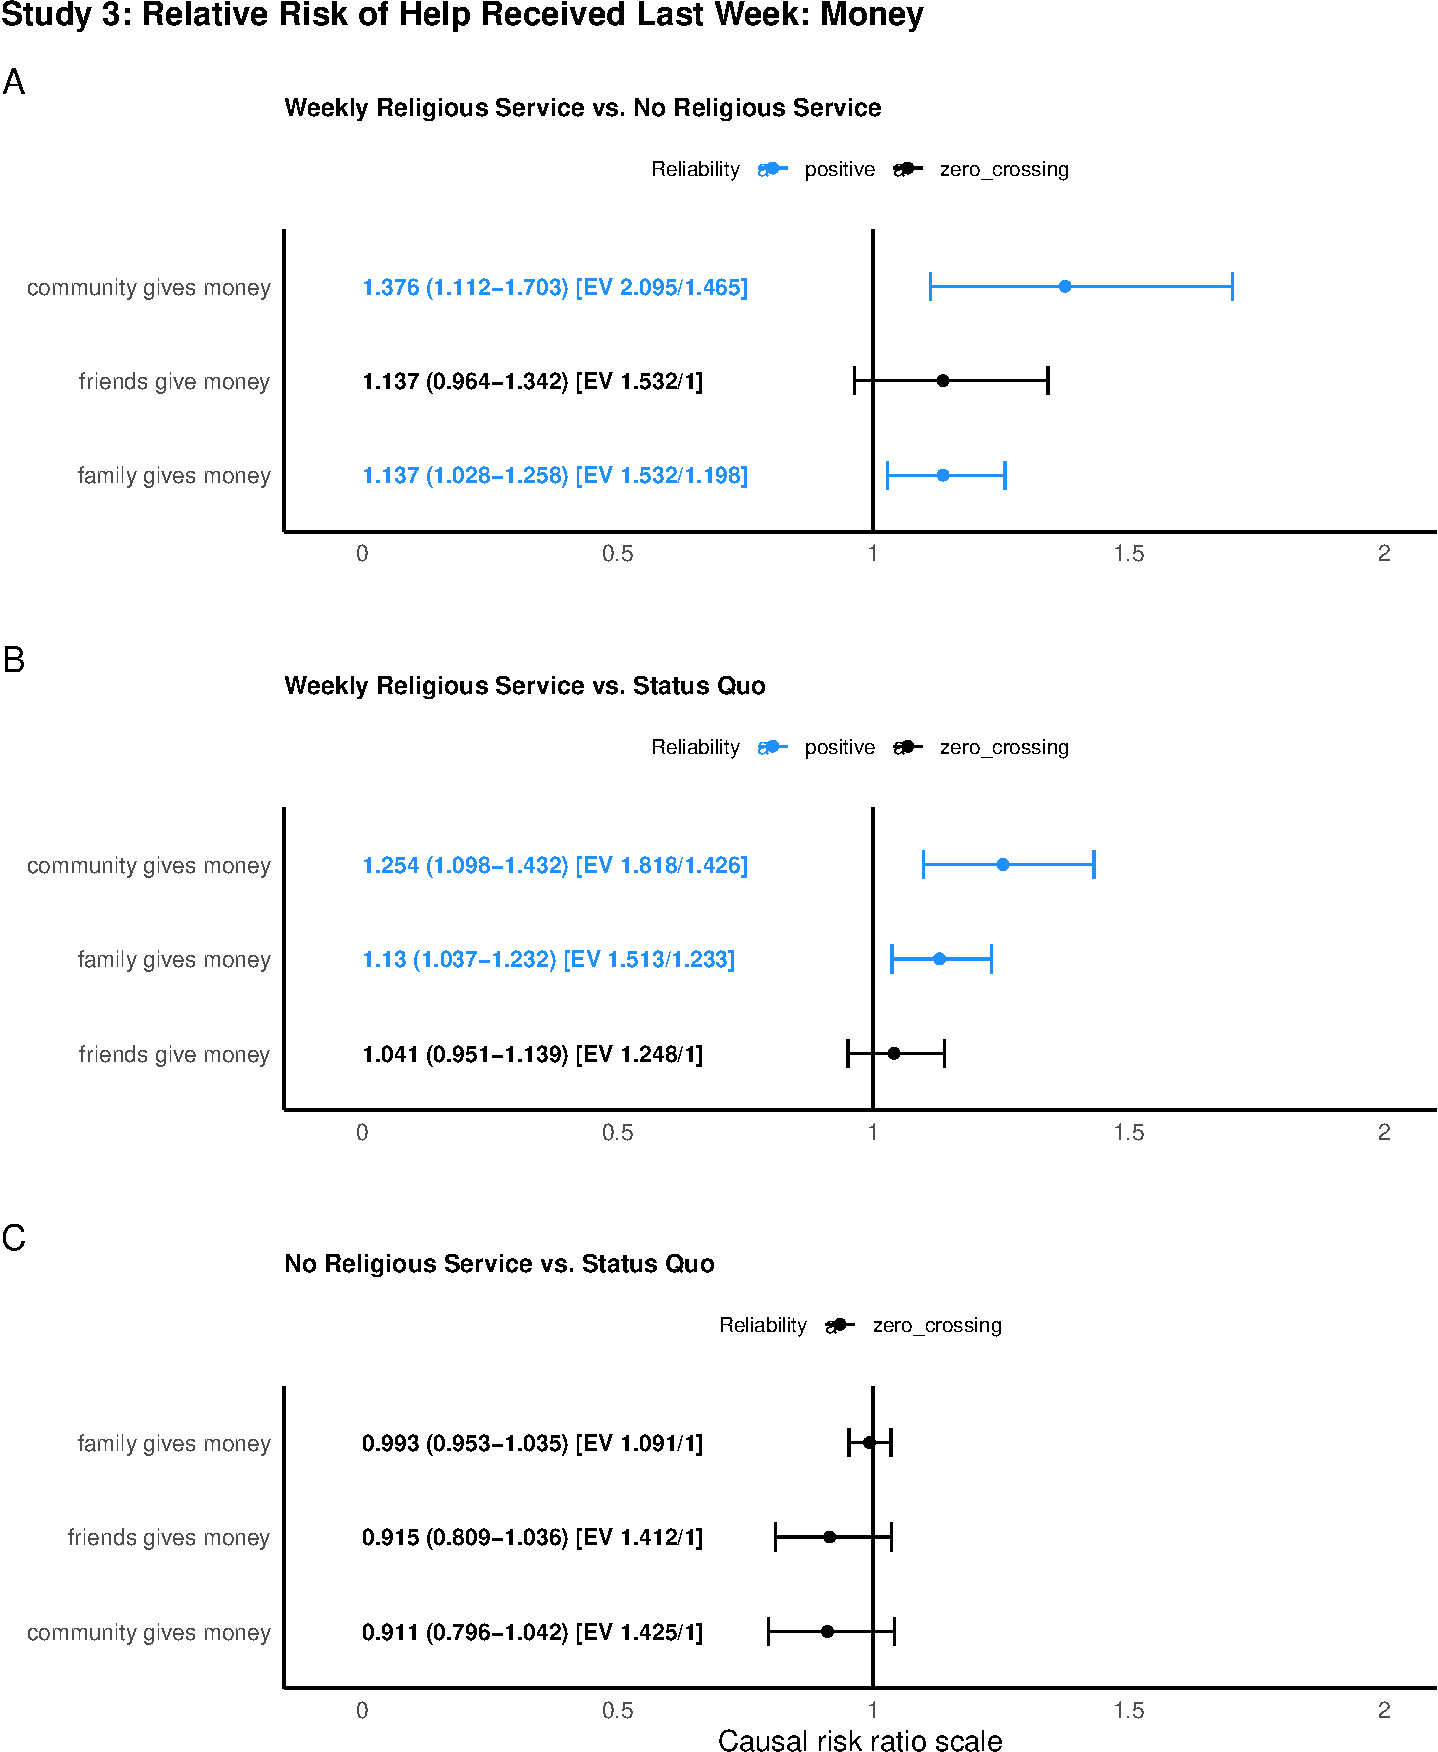
\includegraphics{test_files/figure-pdf/fig-study_3-1.pdf}

}

\caption{\label{fig-study_3}This figure reports the results of model
estimates for the three causal contrasts of interest on help received
from others during the past week (yes/no). The causal contrasts are: (A)
Regular vs.~Zero Religious Service (B) Regular Religious Service
vs.~Status Quo; (C) Zero Religious Service vs.~Status Quo. Contrasts are
expressed on the risk ratio scale.}

\end{figure}%

\newpage{}

\subsubsection{Additional Study: Comparison of Causal Inference Results
with Cross-Sectional
Regressions}\label{additional-study-comparison-of-causal-inference-results-with-cross-sectional-regressions}

To better evaluate the contributions of our methodology to current
practice, we conducted a series of cross-sectional analyses using the
baseline wave data. We quantified the statistical associations between
religious service attendance and our focal prosocial outcomes. We
included all regression covariates from the causal models (including
sample weights) for each analysis, obviously omitting the outcome
measured at baseline, i.e.~the response variable.

\textbf{Cross-sectional volunteering result}: the change in expected
hours of volunteer work for a one-unit increase in religious service
attendance is b = 0.31; (95\% CI 0.28, 0.34). Multiplying this by 4.2
gives a monthly estimate of 77.95 minutes. This result is 2.58 per cent
greater than the effect estimated from the `regular vs.~zero' causal
contrast, indicating an \textbf{overstatement in the cross-sectional
regression model.}

\textbf{Cross-sectional charitable donations result}: The coefficient
for religious service on annual charitable donations suggests a change
in expected donation amount per unit increase in attendance is: b = 451;
(95\% CI 408, 494). When adjusted to a monthly rate by multiplying by
4.2, this value equals NZ Dollars 1894.45. It is 2.89 per cent greater
than our causal contrast estimate, again indicating
\textbf{overstatement in the cross-sectional regression model.}

For Studies 2 and 3, which focus on community help received, we adjusted
our analysis for the non-collapsibility of odds ratios by assuming a
Poisson distribution for the outcome variables, obtaining a rate ratio
that approximates a risk ratio
(\citeproc{ref-huitfeldt2019collapsibility}{Huitfeldt, Stensrud, and
Suzuki 2019}; \citeproc{ref-vanderweele2020}{Tyler J. VanderWeele,
Mathur, and Chen 2020}):

\textbf{Cross-sectional community assistance received result: Time}: the
exponentiated change in expectation for a one-unit change in religious
service attendance is b = 1.17; (95\% CI 1.14, 1.19) approximate risk
rate ratio. The monthly rate ratio derived by multiplying this
coefficient by 4.2 is 1.921. This estimate is 1.39 per cent greater than
the `regular vs.~zero' causal estimate, pointing to
\textbf{overstatement in the cross-sectional regression model.}

\textbf{Cross-sectional community assistance received result: Money}:
similarly, the exponentiated change for money received yields an
approximate risk ratio of b = 1.18; (95\% CI 1.08, 1.27). The monthly
risk ratio, after adjustment, is 1.996. This rate ratio is 1.45 per cent
greater than the causal estimate, again revealing an
\textbf{overstatement in the cross-sectional regression model.}

\emph{These findings underscore that the results of cross-sectional
regressions, although suggestive, can considerably diverge from those
obtained from the causal analysis of panel data.}

\newpage{}

\subsubsection{What is the ``Cash Value'' of Religious Service
Attendance for Charitable Donations in New
Zealand?}\label{what-is-the-cash-value-of-religious-service-attendance-for-charitable-donations-in-new-zealand}

We leveraged results to estimate the approximate economic value of
religious service attendance under different scenarios--- `Regular
Religious Service', `Zero Religious Service', and the `Status Quo',
focusing on charitable donations.

\begin{itemize}
\tightlist
\item
  \textbf{Regular Religious Service}: an increase in religious service
  attendance yields an individual average donation sum of \textbf{NZD
  1638.98.}
\item
  \textbf{Zero Religious Service}: Reducing religious service attendance
  to zero yields an average donation sum of \textbf{NZD 984.59.}
\item
  \textbf{Status Quo}: the expected individual average donation sum is
  currently \textbf{NZD 1037.14.}
\end{itemize}

With 3,989,000 adult residents in New Zealand in 2021:\footnote{\href{https://www.stats.govt.nz/information-releases/national-population-estimates-at-30-june-2021}{National
  Population Estimates at 30 June 2021}}

\begin{itemize}
\tightlist
\item
  Multiplying the adult population by the average donation sum gives a
  status quo national estimate for charitable giving of \textbf{NZD
  4,137,151,460.}
\item
  The net gain to charity from country-wide regular attendance at
  religious services, compared to the status quo, is \textbf{NZD
  2,400,739,760.}
\item
  Conversely, although the net cost to charity from a complete cessation
  of regular religious service attendance is NZD -209,621,950, recall
  the confidence interval crosses zero, and this effect is not reliable.
\end{itemize}

To provide context, consider these economic consequences against the New
Zealand government's annual budget in year outcomes were measured
(2021-2022) is NZD 57,976,000,000

\begin{itemize}
\tightlist
\item
  \textbf{The expected gain from a nationwide adoption of regular
  religious service represents 4.1 percent of New Zealand's annual
  government budget 2021.}
\item
  We do not obtain a reliable effect from the loss intervention.
\end{itemize}

Thus, focussing on the individual-level and aggregating effects across
the adult population, the counterfactual scenario in which all New
Zealand adults regularly attend religious services projects a
substantial increase in society-wide charitable support compared to the
status quo, one year after the intervention.

However, suppose New Zealand were to experience a complete cessation of
religious service attendance. We do not find evidence that the landscape
of charitable giving would change from its current state one year
later.\footnote{We emphasise that failure to rule out an effect is not
  the same as ruling it out. The relatively low levels of religious
  service attendance in New Zealand mutes differences in expected
  giving. In our view, some amount of charity is always better than
  none. We do not devalue any form of charitable giving. Furthermore,
  our population-wide estimates for the aggregated effects of
  \emph{religious behaviour} do not clarify the effects of gaining or
  losing \emph{religious institutions}; our analysis reflects the
  contributions made by those participating in religious institutions.}

\subsection{Discussion}\label{discussion}

\subsubsection{Considerations}\label{considerations}

First, as stated above, our causal inferences turn on three assumptions,
which are worth revisiting:

(i). \textbf{Unmeasured confounding}: although we employ robust methods
for causal inference, our results depend on the effectiveness of our
strategy to control for confounding. Our sensitivity analyses address
the potential impacts of unmeasured confounders. Nevertheless, the
presence and influence of such confounders are uncertain and
unverifiable from our data.

(ii). \textbf{Causal consistency}: the observed outcomes must correspond
to the counterfactual treatments contrasted. Although ``religious
service attendance'' may appear conditionally independent of the
outcomes given baseline covariates, interpreting these interventions
remains challenging. ``Religious service attendance'' varies widely,
encompassing everything from informal gatherings at homes to formal
services in cathedrals across New Zealand's religious diversity. This
type of ``treatment'' does not mirror a straightforward medical
intervention like a vaccine. The heterogeneity of ``religious service''
limits the clarity of our results, an issue no amount of data or
analysis can resolve because ``religious service'' reflects a broad
spectrum of community activities.

(iii). \textbf{Positivity}: we have confirmed that religious service
attendance varies within our sample and have used semi-parametric models
with ensemble learning and cross-validation to prevent data
over-extrapolation and model over-fitting. Conceptually, it is crucial
for valid causal inference that every potential level of ``treatment''
to religious services is realistically possible (refer to discussion in
Tyler J. VanderWeele
(\citeproc{ref-vanderweele2017causaleffectsService}{2017})). Although
there are instances realised in our data of secular individuals
initiating religious service and frequent attendees stopping (refer to
Table~\ref{tbl-transition}), it might stretch credulity too far to
imagine that such changes are possible for everyone.

Second, our study confronts the spectre of \textbf{measurement error}:
both direct and correlated measurement errors can introduce biases,
either by implying effects where none exist or by attenuating true
effects (\citeproc{ref-vanderweele2012MEASUREMENT}{Tyler J. VanderWeele
and Hernán 2012}). Importantly, evaluating prosociality using multiple
measures while also controlling for these measures and the treatment at
baseline helps to mitigate measurement error concerns. Nevertheless,
unknown combinations of measurement error might nevertheless bias our
results. The outcomes and estimates we report here are best-considered
approximations.

Third, we do not examine \textbf{treatment effect heterogeneity}:
identifying which subgroups experience the strongest responses remains a
task for future research. Such investigations are crucial for making
informed policy decisions and tailoring advice relevant to those
subgroups of the population who might benefit most. Perhaps the most
obvious stratum is religious affiliates
(\citeproc{ref-vanderweele2017causaleffectsService}{Tyler J. VanderWeele
2017}).

Fourth, the \textbf{transportability of our findings remains unclear}:
New Zealand is our target population. Our findings generalise to this
population. However, the transportability of our findings to other
settings---whether our results generalise beyond our targeted New
Zealand population---remains an open question, a matter for future
investigations.

\subsubsection{Observations and
Recommendations}\label{observations-and-recommendations}

First, it is essential to notice that ``Does religion cause
prosociality?'' lacks specificity. To refine this question, we must
articulate clear causal contrasts and their scale, select specific
measures of ``prosociality,'' define our target population, gather
appropriate time-series data, and, only after causal assumptions and
identification criteria are satisfied and threats made explicit,
calculate statistical estimates. Having obtained these estimates, which
rely on assumptions, we must evaluate robustness using sensitivity
analyses (\citeproc{ref-hernan2024WHATIF}{Hernan and Robins 2024};
\citeproc{ref-ogburn2021}{Ogburn and Shpitser 2021};
\citeproc{ref-bulbulia2022}{J. A. Bulbulia 2022};
\citeproc{ref-linden2020EVALUE}{Linden, Mathur, and VanderWeele 2020};
\citeproc{ref-vanderweele2020}{Tyler J. VanderWeele, Mathur, and Chen
2020}).

Here, we obtain statistical estimates for the causal effects of
religious service on charity and volunteering by (1) stating contrasts
for specific interventions that increase and decrease religious service
attendance across the population; (2) balancing the interventions to be
compared on baseline confounders measured one year before treatment
(including baseline measures of the treatment and outcomes) using
flexible doubly robust machine learning ensembles with cross-validation;
and (3) evaluating contrasts in expected average outcomes under
different treatments one year after treatment.

In the scientifically interesting contrast condition, `Regular vs Zero',
we find considerable social benefits of regular religious attendance for
charitable donations and volunteering. Moreover, we also find that
regular religious service enacted in contemporary New Zealand would
strongly enhance charity and volunteering above the status quo, a point
that may inform discussions among critics of religion. Conversely, the
overall social effects of altogether ceasing religious services are
minimal compared with the status quo. Were New Zealand society to
entirely forgo regular religious attendance, differences in charitable
donations and volunteering one year later are unreliable. Although we
did not investigate the long-term effects of the interventions
considered here, this finding should alleviate some concerns among those
wary of New Zealand's longstanding secular trend. Looking ahead,
\textbf{we recommend that future research distinguish between models of
treatment-gain and models of treatment-loss} (as exemplified by Van
Tongeren et al. (\citeproc{ref-vantongeren2020}{2020})).

Second, we caution that \textbf{classical measures of effect, such as
Cohen's \emph{D} or \(R^2\), may present a misleading indication of
practical significance.} Our study computed standardised differences in
the continuous charity and volunteering outcomes. The contrast between
regular religious service and no service yields and effects size of
0.132 {[}0.102, 0.161{]}. This effect would be categorised as ``small''
effect by contemporary experimental conventions. Nonetheless, we project
that the difference in annual charitable donations between the regular
service condition and the status quo amounts to NZD 1638.98 versus NZD
1037.14. Not only is this effect practically significant at the
individual level, summed over the population the difference amounts to
4\% of New Zealand's Annual Government Budget (2021). \textbf{We
recommend using causal inference to prioritise, evaluate and communicate
practical effect sizes. Conventional statistical measures should not be
mistaken for metrics of practical significance.}

Third, our novel measures of prosociality---\textbf{assistance and
financial support received from one's community}--align with the
expectations of self-reported data on charitable donations and
volunteering. We detect marginal causal effects of religious service
attendance on \textbf{measures of prosocial benefit and dependence}.
Notice that just as our measures of prosocial actions
(charity/volunteering) do not capture the targets of prosocial help,
likewise our measures of community help received (time/money) do not
capture the specific sources of help beyond the categories of
``community,'' ``friends,'' and ``family''. Nevertheless, the
evolutionary theories of religious prosociality that motivate this study
are grounded on within-group cooperative benefits
(\citeproc{ref-sosis2003cooperation}{Sosis and Bressler 2003};
\citeproc{ref-johnson2015}{D. D. Johnson 2015};
\citeproc{ref-bulbulia2012spreading}{J. Bulbulia 2012};
\citeproc{ref-whitehouse2023}{Whitehouse et al. 2023};
\citeproc{ref-schloss2011evolutionary}{Schloss and Murray 2011}). This
consistency between self-reported giving and help received aligns with
public data in New Zealand;\footnote{\url{https://www.charities.govt.nz/view-data/}}
where religious institutional charity accounts for 40\% of the
charitable sector (refer to McLeod (\citeproc{ref-McLeod2020}{2020}),
p.17, and also Brooks (\citeproc{ref-brooks2004faith}{2004}); Woodyard
and Grable (\citeproc{ref-woodyard2014doing}{2014}); Monsma
(\citeproc{ref-monsma2007religion}{2007})). Additionally, religious
institutions appear particularly efficient owing to low administrative
costs and high volunteer engagement
(\citeproc{ref-khanna1995charity}{Khanna, Posnett, and Sandler 1995};
\citeproc{ref-bekkers2011literature}{Bekkers and Wiepking 2011};
\citeproc{ref-McLeod2020}{McLeod 2020, 26}). We note that the community
signals of religious giving are consistent with the theory that religion
promotes altruism outside families, friendships, and even among
strangers (\citeproc{ref-mccullough2020kindness}{McCullough 2020}).
\textbf{In contexts where investigators are concerned about
self-presentation biases when surveying charitable donations and
volunteering, we recommend piloting and deploying measures that capture
community-received assistance.}

Fourth, our secondary analysis reveals that standard cross-sectional
regressions overstate the causal effects estimates obtained from a
conscientious application of causal methods to time-series data.
Importantly, associational models might also \emph{understate} true
causal relationships, especially if adjustments involve mediators
(\citeproc{ref-westreich2013}{Westreich and Greenland 2013};
\citeproc{ref-mcelreath2020}{McElreath 2020}). Despite their
effectiveness and relevance, causal inference methods remain uncommon in
many human sciences, including the psychological sciences, where
traditional associational methods still dominate. Transitioning to
causal data science might seem daunting. Yet, causation inherently
unfolds in time, with causes preceding effects. Estimating average
causal effects involves multi-stepped workflows and robust time-series
data (\citeproc{ref-neal2020introduction}{Neal 2020};
\citeproc{ref-bulbulia2023}{J. A. Bulbulia 2023}). Although the need for
researchers to develop new skills imposes considerable demands, it is
encouraging that methods for causal inference have become standard in
epidemiology (\citeproc{ref-lash2020}{Lash et al. 2020}) and are rapidly
gaining traction in economics (\citeproc{ref-angrist2009mostly}{Angrist
and Pischke 2009}; \citeproc{ref-athey2019}{Athey, Tibshirani, and Wager
2019}; \citeproc{ref-athey2021}{Athey and Wager 2021}) and political
science (\citeproc{ref-montgomery2018}{Montgomery, Nyhan, and Torres
2018}).

Moreover, a global panel studies suited for researching religion B. R.
Johnson and VanderWeele (\citeproc{ref-johnson2022global}{2022}) offers
exciting opportunities for psychological scientists to apply causal
methods to those psychological questions at the heart of our discipline.

Also encouraging, well-designed panel studies investigating the causal
effects of religious service attendance on health that capitalise on the
affordances of time-series data provide models for studies that may
investigate the social consequences of religion (refer to Y. Chen, Kim,
and VanderWeele (\citeproc{ref-chen2020religious}{2020}), Pawlikowski et
al. (\citeproc{ref-pawlikowski2019religious}{2019}),Li et al.
(\citeproc{ref-vanderweelechurchmortality}{2016}),Tyler J. VanderWeele
(\citeproc{ref-vanderweele2021effectsReligiousServiceMetanalysis}{2021b}),
Kim and VanderWeele (\citeproc{ref-kim2019mediators}{2019})). At
present, then, the intellectual benefits of retooling would seem
considerable (refer to Major-Smith
(\citeproc{ref-major2023exploring}{2023})).

Setting intellectual benefits aside, it is vital to remember that
investigators should be able to evaluate the practical interest of their
findings coherently. Such evaluation relies on quantifying the effects
of interventions. However, associational methods cannot deliver this
understanding where causal inferential workflows are absent because
association is not guaranteed to be causation
(\citeproc{ref-westreich2013}{Westreich and Greenland 2013}). What might
be called a \emph{practical significance gap} arises from associational
models because we cannot interpret associations as causation unless we
have obtained balance on the treatments to be compared, know that causes
in our data precede effects in time, and ensure that identification
conditions have been met. Notably, the \emph{practical significance gap}
remains for associational methods even when they are applied to time
series data, and even when they are sophisticated---as in the
statistical structural equation and multilevel modelling traditions
(refer to Tyler J. VanderWeele
(\citeproc{ref-vanderweele2021can}{2021a}); Hazlett and Wainstein
(\citeproc{ref-hazlett2022understanding}{2022})). Yet, because
investigators typically seek both scientific knowledge and practical
understanding, \textbf{we strongly recommend the broader adoption of
causal inferential methods in the psychological sciences.}

Fifth, and finally, we frame this study's contribution in light of
future horizons. This study combined robust causal methods with national
panel data to quantitatively investigate the social consequences of
religious behaviour. Using both stated and revealed indicators, we
provide evidence that religious service attendance causally affects
charitable donations and volunteering. These findings offer insights
into \emph{how much} Religious service affects charity and volunteering
in New Zealand and possibly in similar cultures. We hope this research
will serve as a guide for studies in other settings.

However, even within New Zealand, much remains to be discovered. We have
not attempted to elucidate heterogeneity in the treatment effects we
observe. Nor have we investigated the pathways by which religious
service attendance affects social behaviours. A substantial body of
research has examined the psychological and cultural features through
which religious behaviours affect individuals
(\citeproc{ref-norenzayan2016}{Norenzayan et al. 2016};
\citeproc{ref-shaver2020church}{Shaver et al. 2020};
\citeproc{ref-watts2016}{J. Watts et al. 2016};
\citeproc{ref-mccullough2016christian}{McCullough et al. 2016};
\citeproc{ref-konvalinka2011synchronized}{Konvalinka et al. 2011};
\citeproc{ref-lang2015effects}{Lang et al. 2015};
\citeproc{ref-cristofori2016neural}{Cristofori et al. 2016};
\citeproc{ref-shaver2015evolution}{Shaver 2015};
\citeproc{ref-sosis2005does}{Sosis 2005}). Yet obtaining a causal
understanding presents conceptual, modelling, and data challenges
(\citeproc{ref-robins1992}{J. M. Robins and Greenland 1992};
\citeproc{ref-vanderweele2015}{Tyler J. VanderWeele 2015};
\citeproc{ref-Diaz2023}{Dı́az, Williams, and Rudolph 2023};
\citeproc{ref-diaz2021nonparametric}{Dı́az et al. 2021}). In the years
ahead, \textbf{we recommend the wider development and application of
causal inferential methods employing repeated measurements over more
than three years to investigate variation, interaction, and causal
mediation}.

\newpage{}

\subsubsection{Ethics}\label{ethics}

The University of Auckland Human Participants Ethics Committee reviews
the NZAVS every three years. Our most recent ethics approval statement
is as follows: The New Zealand Attitudes and Values Study was approved
by the University of Auckland Human Participants Ethics Committee on
26/05/2021 for six years until 26/05/2027, Reference Number UAHPEC22576.

\subsubsection{Data Availability}\label{data-availability}

The data described in the paper are part of the New Zealand Attitudes
and Values Study (NZAVMembers of the NZAVS management team and research
group hold full copies of the NZAVS data. A de-identified dataset
containing only the variables analysed in this manuscript is available
upon request from the corresponding author or any member of the NZAVS
advisory board for replication or checking of any published study using
NZAVS data. The code for the analysis can be found at:
\url{https://github.com/go-bayes/models/blob/main/scripts/24-bulbulia-church-prosocial.R}.

\newpage{}

\subsection{Appendix A: Measures}\label{appendix-measures}

\paragraph{Age (waves: 1-15)}\label{age-waves-1-15}

We asked participants' ages in an open-ended question (``What is your
age?'' or ``What is your date of birth?'').

\paragraph{Born in New Zealand}\label{born-in-new-zealand}

\paragraph{Charitable Donations (Study 1
outcome)}\label{charitable-donations-study-1-outcome}

Using one item from Hoverd and Sibley
(\citeproc{ref-hoverd_religious_2010}{2010}), we asked participants,
``How much money have you donated to charity in the last year?''.

\paragraph{Charitable Volunteering (Study 1
outcome)}\label{charitable-volunteering-study-1-outcome}

We measured hours of volunteering using one item from Chris G. Sibley et
al. (\citeproc{ref-sibley2011}{2011}): ``Hours spent \ldots{}
voluntary/charitable work.''

\paragraph{Children Number (waves: 1-3,
4-15)}\label{children-number-waves-1-3-4-15}

We measured the number of children using one item from J. A. Bulbulia et
al. (\citeproc{ref-Bulbulia_2015}{2015}). We asked participants, ``How
many children have you given birth to, fathered, or adopted. How many
children have you given birth to, fathered, or adopted?'' or ``How many
children have you given birth to, fathered, or adopted. How many
children have you given birth to, fathered, and/or parented?'' (waves:
12-15).

\paragraph{Disability}\label{disability}

We assessed disability with a one-item indicator adapted from Verbrugge
(\citeproc{ref-verbrugge1997}{1997}). It asks, ``Do you have a health
condition or disability that limits you and that has lasted for 6+
months?'' (1 = Yes, 0 = No).

\paragraph{Education Attainment (waves: 1,
4-15)}\label{education-attainment-waves-1-4-15}

We asked participants, ``What is your highest level of qualification?''.
We coded participants' highest finished degree according to the New
Zealand Qualifications Authority. Ordinal-Rank 0-10 NZREG codes (with
overseas school quals coded as Level 3, and all other ancillary
categories coded as missing)
See:https://www.nzqa.govt.nz/assets/Studying-in-NZ/New-Zealand-Qualification-Framework/requirements-nzqf.pdf

\paragraph{Employment (waves: 1-3,
4-11)}\label{employment-waves-1-3-4-11}

We asked participants, ``Are you currently employed? (This includes
self-employed or casual work)''.

\paragraph{Ethnicity}\label{ethnicity}

Based on the New Zealand Census, we asked participants, ``Which ethnic
group(s) do you belong to?''. The responses were: (1) New Zealand
European; (2) Māori; (3) Samoan; (4) Cook Island Māori; (5) Tongan; (6)
Niuean; (7) Chinese; (8) Indian; (9) Other such as DUTCH, JAPANESE,
TOKELAUAN. Please state:. We coded their answers into four groups:
Maori, Pacific, Asian, and Euro (except for Time 3, which used an
open-ended measure).

\paragraph{Fatigue}\label{fatigue}

We assessed subjective fatigue by asking participants, ``During the last
30 days, how often did \ldots{} you feel exhausted?'' Responses were
collected on an ordinal scale (0 = None of The Time, 1 = A little of The
Time, 2 = Some of The Time, 3 = Most of The Time, 4 = All of The Time).

\paragraph{Honesty-Humility-Modesty Facet (waves:
10-14)}\label{honesty-humility-modesty-facet-waves-10-14}

Participants indicated the extent to which they agree with the following
four statements from Campbell et al. (\citeproc{ref-campbell2004}{2004})
, and Chris G. Sibley et al. (\citeproc{ref-sibley2011}{2011}) (1 =
Strongly Disagree to 7 = Strongly Agree)

\begin{verbatim}
i.  I want people to know that I am an important person of high status, (Waves: 1, 10-14)
ii. I am an ordinary person who is no better than others.
iii. I wouldn't want people to treat me as though I were superior to them.
iv. I think that I am entitled to more respect than the average person is.
\end{verbatim}

\paragraph{Hours of Childcare}\label{hours-of-childcare}

We measured hours of exercising using one item from Chris G. Sibley et
al. (\citeproc{ref-sibley2011}{2011}): 'Hours spent \ldots{} looking
after children.''

To stabilise this indicator, we took the natural log of the response +
1.

\paragraph{Hours of Housework}\label{hours-of-housework}

We measured hours of exercising using one item from Chris G. Sibley et
al. (\citeproc{ref-sibley2011}{2011}): ``Hours spent \ldots{}
housework/cooking''

To stabilise this indicator, we took the natural log of the response +
1.

\paragraph{Hours of Exercise}\label{hours-of-exercise}

We measured hours of exercising using one item from Chris G. Sibley et
al. (\citeproc{ref-sibley2011}{2011}): ``Hours spent \ldots{}
exercising/physical activity''

To stabilise this indicator, we took the natural log of the response +
1.

\paragraph{Hours of Childcare}\label{hours-of-childcare-1}

We measured hours of exercising using one item from Chris G. Sibley et
al. (\citeproc{ref-sibley2011}{2011}): 'Hours spent \ldots{} looking
after children.''

To stabilise this indicator, we took the natural log of the response +
1.

\paragraph{Hours of Exercise}\label{hours-of-exercise-1}

We measured hours of exercising using one item from Chris G. Sibley et
al. (\citeproc{ref-sibley2011}{2011}): ``Hours spent \ldots{}
exercising/physical activity''

To stabilise this indicator, we took the natural log of the response +
1.

\paragraph{Hours of Housework}\label{hours-of-housework-1}

We measured hours of exercising using one item from Chris G. Sibley et
al. (\citeproc{ref-sibley2011}{2011}): ``Hours spent \ldots{}
housework/cooking''

To stabilise this indicator, we took the natural log of the response +
1.

\paragraph{Hours of Sleep}\label{hours-of-sleep}

Participants were asked, ``During the past month, on average, how many
hours of \emph{actual sleep} did you get per night?''.

\paragraph{Hours of Work}\label{hours-of-work}

We measured work hours using one item from Chris G. Sibley et al.
(\citeproc{ref-sibley2011}{2011}): ``Hours spent \ldots{} working in
paid employment.''

To stabilise this indicator, we took the natural log of the response +
1.

\paragraph{Income (waves: 1-3, 4-15)}\label{income-waves-1-3-4-15}

Participants were asked, ``Please estimate your total household income
(before tax) for the year XXXX''. To stabilise this indicator, we first
took the natural log of the response + 1, and then centred and
standardised the log-transformed indicator.

\paragraph{Kessler-6: Psychological Distress (waves:
2-3,4-15)}\label{kessler-6-psychological-distress-waves-2-34-15}

We measured psychological distress using the Kessler-6 scale
(kessler2002?), which exhibits strong diagnostic concordance for
moderate and severe psychological distress in large, crosscultural
samples (kessler2010?; prochaska2012?). Participants rated during the
past 30 days, how often did\ldots{} (1) ``\ldots{} you feel hopeless'';
(2) ``\ldots{} you feel so depressed that nothing could cheer you up'';
(3) ``\ldots{} you feel restless or fidgety''; (4)``\ldots{} you feel
that everything was an effort''; (5) ``\ldots{} you feel worthless'';
(6) '' you feel nervous?'' Ordinal response alternatives for the
Kessler-6 are: ``None of the time''; ``A little of the time''; ``Some of
the time''; ``Most of the time''; ``All of the time.''

\paragraph{Male Gender (waves: 1-15)}\label{male-gender-waves-1-15}

We asked participants' gender in an open-ended question: ``what is your
gender?'' or ``Are you male or female?'' (waves: 1-5). Female was coded
as 0, Male as 1, and gender diverse coded as 3
(\citeproc{ref-fraser_coding_2020}{Fraser et al. 2020}). (or 0.5 =
neither female nor male)

Here, we coded all those who responded as Male as 1, and those who did
not as 0.

\paragraph{Mini-IPIP 6 (waves:
1-3,4-15)}\label{mini-ipip-6-waves-1-34-15}

We measured participants' personalities with the Mini International
Personality Item Pool 6 (Mini-IPIP6) (\citeproc{ref-sibley2011}{Chris G.
Sibley et al. 2011}), which consists of six dimensions and each
dimension is measured with four items:

\begin{enumerate}
\def\labelenumi{\arabic{enumi}.}
\item
  agreeableness,

  \begin{enumerate}
  \def\labelenumii{\roman{enumii}.}
  \tightlist
  \item
    I sympathize with others' feelings.
  \item
    I am not interested in other people's problems. (r)
  \item
    I feel others' emotions.
  \item
    I am not really interested in others. (r)
  \end{enumerate}
\item
  conscientiousness,

  \begin{enumerate}
  \def\labelenumii{\roman{enumii}.}
  \tightlist
  \item
    I get chores done right away.
  \item
    I like order.
  \item
    I make a mess of things. (r)
  \item
    I often forget to put things back in their proper place. (r)
  \end{enumerate}
\item
  extraversion,

  \begin{enumerate}
  \def\labelenumii{\roman{enumii}.}
  \tightlist
  \item
    I am the life of the party.
  \item
    I don't talk a lot. (r)
  \item
    I keep in the background. (r)
  \item
    I talk to a lot of different people at parties.
  \end{enumerate}
\item
  honesty-humility,

  \begin{enumerate}
  \def\labelenumii{\roman{enumii}.}
  \tightlist
  \item
    I feel entitled to more of everything. (r)
  \item
    I deserve more things in life. (r)
  \item
    I would like to be seen driving around in a very expensive car. (r)
  \item
    I would get a lot of pleasure from owning expensive luxury goods.
    (r)
  \end{enumerate}
\item
  neuroticism, and

  \begin{enumerate}
  \def\labelenumii{\roman{enumii}.}
  \tightlist
  \item
    I have frequent mood swings.
  \item
    I am relaxed most of the time. (r)
  \item
    I get upset easily.
  \item
    I seldom feel blue. (r)
  \end{enumerate}
\item
  openness to experience

  \begin{enumerate}
  \def\labelenumii{\roman{enumii}.}
  \tightlist
  \item
    I have a vivid imagination.
  \item
    I have difficulty understanding abstract ideas. (r)
  \item
    I do not have a good imagination. (r)
  \item
    I am not interested in abstract ideas. (r)
  \end{enumerate}
\end{enumerate}

Each dimension was assessed with four items and participants rated the
accuracy of each item as it applies to them from 1 (Very Inaccurate) to
7 (Very Accurate). Items marked with (r) are reverse coded.

\paragraph{NZ-Born (waves: 1-2,4-15)}\label{nz-born-waves-1-24-15}

We asked participants, ``Which country were you born in?'' or ``Where
were you born? (please be specific, e.g., which town/city?)'' (waves:
6-15).

\paragraph{NZ Deprivation Index (waves:
1-15)}\label{nz-deprivation-index-waves-1-15}

We used the NZ Deprivation Index to assign each participant a score
based on where they live (\citeproc{ref-atkinson2019}{Atkinson, Salmond,
and Crampton 2019}). This score combines data such as income, home
ownership, employment, qualifications, family structure, housing, and
access to transport and communication for an area into one deprivation
score.

\paragraph{NZSEI Occupational Prestige and Status (waves:
8-15)}\label{nzsei-occupational-prestige-and-status-waves-8-15}

We assessed occupational prestige and status using the New Zealand
Socio-economic Index 13 (NZSEI-13) (\citeproc{ref-fahy2017a}{Fahy, Lee,
and Milne 2017a}). This index uses the income, age, and education of a
reference group, in this case the 2013 New Zealand census, to calculate
a score for each occupational group. Scores range from 10 (Lowest) to 90
(Highest). This list of index scores for occupational groups was used to
assign each participant an NZSEI-13 score based on their occupation.

We assessed occupational prestige and status using the New Zealand
Socio-economic Index 13 (NZSEI-13) (\citeproc{ref-fahy2017}{Fahy, Lee,
and Milne 2017b}). This index uses the income, age, and education of a
reference group, in this case, the 2013 New Zealand census, to calculate
a score for each occupational group. Scores range from 10 (Lowest) to 90
(Highest). This list of index scores for occupational groups was used to
assign each participant an NZSEI-13 score based on their occupation.

\paragraph{Opt-in}\label{opt-in}

The New Zealand Attitudes and Values Study allows opt-ins to the study.
Because the opt-in population may differ from those sampled randomly
from the New Zealand electoral roll; although the opt-in rate is low, we
include an indicator (yes/no) for this variable.

\paragraph{Partner (No/Yes)}\label{partner-noyes}

``What is your relationship status?'' (e.g., single, married, de-facto,
civil union, widowed, living together, etc.)

\paragraph{Politically Conservative}\label{politically-conservative}

We measured participants' political conservative orientation using a
single item adapted from Jost (\citeproc{ref-jost_end_2006-1}{2006}).

``Please rate how politically liberal versus conservative you see
yourself as being.''

(1 = Extremely Liberal to 7 = Extremely Conservative)

\subparagraph{Religious Service
Attendance}\label{religious-service-attendance}

If participants answered \emph{yes} to ``Do you identify with a religion
and/or spiritual group?'' we measured their frequency of church
attendence using one item from Sibley C. G. and Bulbulia
(\citeproc{ref-sibley2012}{2012}): ``how many times did you attend a
church or place of worship in the last month?''. Those participants who
were not religious were imputed a score of ``0''.

\paragraph{Rural/Urban Codes}\label{ruralurban-codes}

Participants residence locations were coded according to a five-level
ordinal categorisation ranging from ``Urban'' to Rural, see Chris G.
Sibley (\citeproc{ref-sibley2021}{2021}).

\paragraph{Short-Form Health}\label{short-form-health}

Participants' subjective health was measured using one item (``Do you
have a health condition or disability that limits you, and that has
lasted for 6+ months?''; 1 = Yes, 0 = No) adapted from Verbrugge
(\citeproc{ref-verbrugge1997}{1997}).

\paragraph{Sample Origin}\label{sample-origin}

Wave enrolled in NZAVS, see Chris G. Sibley
(\citeproc{ref-sibley2021}{2021}).

\paragraph{Support received: money (waves 10-12) (Study 4
outcomes)}\label{support-received-money-waves-10-12-study-4-outcomes}

The NZAVS has a `revealed' measure of received help and support measured
in hours of support in the previous week. The items are:

\emph{Please estimate how much help you have received from the following
sources in the last week?}

\begin{itemize}
\tightlist
\item
  \emph{family\ldots MONEY (hours)}
\item
  \emph{friends\ldots MONEY (hours)}
\item
  \emph{members of my community\ldots MONEY (hours)}
\end{itemize}

Because this measure is highly variable, we convert responses to binary
indicators: \emph{0 = none/1 any}

\paragraph{Support received: time (waves 10-13) (Study 3
outcomes)}\label{support-received-time-waves-10-13-study-3-outcomes}

\emph{Please estimate how much help you have received from the following
sources in the last week.}

\begin{itemize}
\tightlist
\item
  \emph{family\ldots TIME (hours)}
\item
  \emph{friends\ldots TIME (hours)}
\item
  \emph{members of my community\ldots TIME (hours)}
\end{itemize}

Because this measure is highly variable, we convert responses to binary
indicators: \emph{0 = none/1 any}

\paragraph{Total Siblings}\label{total-siblings}

Participants were asked the following questions related to sibling
counts:

\begin{itemize}
\tightlist
\item
  Were you the 1st born, 2nd born, or 3rd born, etc, child of your
  mother?
\item
  Do you have siblings?
\item
  How many older sisters do you have?
\item
  How many younger sisters do you have?
\item
  How many older brothers do you have?
\item
  How many younger brothers do you have?
\end{itemize}

A single score was obtained from sibling counts by summing responses to
the ``How many\ldots{}'' items. From these scores, an ordered factor was
created ranging from 0 to 7, where participants with more than 7
siblings were grouped into the highest category.

\newpage{}

\subsection{Appendix B. Baseline Demographic
Statistics}\label{appendix-demographics}

\begin{longtable}[]{@{}ll@{}}

\caption{\label{tbl-table-demography}Baseline demographic statistics}

\tabularnewline

\toprule\noalign{}
\textbf{Exposure + Demographic Variables} & \textbf{N = 33,198} \\
\midrule\noalign{}
\endhead
\bottomrule\noalign{}
\endlastfoot
\textbf{Age} & NA \\
Mean (SD) & 51 (14) \\
Range & 18, 96 \\
IQR & 41, 61 \\
\textbf{Agreeableness} & NA \\
Mean (SD) & 5.37 (0.98) \\
Range & 1.00, 7.00 \\
IQR & 4.75, 6.00 \\
Unknown & 272 \\
\textbf{Born Nz} & 26,197 (79\%) \\
Unknown & 34 \\
\textbf{Children Num} & NA \\
Mean (SD) & 1.76 (1.44) \\
Range & 0.00, 14.00 \\
IQR & 0.00, 3.00 \\
\textbf{Conscientiousness} & NA \\
Mean (SD) & 5.14 (1.04) \\
Range & 1.00, 7.00 \\
IQR & 4.50, 6.00 \\
Unknown & 266 \\
\textbf{Education Level Coarsen} & NA \\
no\_qualification & 769 (2.3\%) \\
cert\_1\_to\_4 & 11,278 (34\%) \\
cert\_5\_to\_6 & 4,281 (13\%) \\
university & 8,947 (27\%) \\
post\_grad & 3,892 (12\%) \\
masters & 2,956 (9.0\%) \\
doctorate & 891 (2.7\%) \\
Unknown & 184 \\
\textbf{Employed} & 26,379 (80\%) \\
Unknown & 26 \\
\textbf{Eth Cat} & NA \\
euro & 27,404 (83\%) \\
maori & 3,424 (10\%) \\
pacific & 707 (2.1\%) \\
asian & 1,438 (4.4\%) \\
Unknown & 225 \\
\textbf{Extraversion} & NA \\
Mean (SD) & 3.88 (1.20) \\
Range & 1.00, 7.00 \\
IQR & 3.00, 4.75 \\
Unknown & 266 \\
\textbf{Hlth Disability} & 7,558 (23\%) \\
Unknown & 561 \\
\textbf{Hlth Fatigue} & NA \\
0 & 5,289 (16\%) \\
1 & 10,940 (33\%) \\
2 & 10,196 (31\%) \\
3 & 4,862 (15\%) \\
4 & 1,577 (4.8\%) \\
Unknown & 334 \\
\textbf{Hlth Sleep Hours} & NA \\
Mean (SD) & 6.95 (1.11) \\
Range & 2.50, 16.00 \\
IQR & 6.00, 8.00 \\
Unknown & 1,528 \\
\textbf{Honesty Humility} & NA \\
Mean (SD) & 5.49 (1.15) \\
Range & 1.00, 7.00 \\
IQR & 4.75, 6.50 \\
Unknown & 269 \\
\textbf{Hours Children log} & NA \\
Mean (SD) & 1.10 (1.58) \\
Range & 0.00, 5.13 \\
IQR & 0.00, 2.20 \\
Unknown & 875 \\
\textbf{Hours Exercise log} & NA \\
Mean (SD) & 1.57 (0.83) \\
Range & 0.00, 4.39 \\
IQR & 1.10, 2.08 \\
Unknown & 875 \\
\textbf{Hours Housework log} & NA \\
Mean (SD) & 2.15 (0.77) \\
Range & 0.00, 5.13 \\
IQR & 1.79, 2.71 \\
Unknown & 875 \\
\textbf{Hours Work log} & NA \\
Mean (SD) & 2.64 (1.59) \\
Range & 0.00, 4.62 \\
IQR & 1.10, 3.71 \\
Unknown & 875 \\
\textbf{Household Inc log} & NA \\
Mean (SD) & 11.41 (0.76) \\
Range & 0.69, 14.92 \\
IQR & 11.00, 11.92 \\
Unknown & 1,352 \\
\textbf{Kessler6 Sum} & NA \\
Mean (SD) & 5 (4) \\
Range & 0, 24 \\
IQR & 2, 7 \\
Unknown & 297 \\
\textbf{Male} & 11,975 (36\%) \\
\textbf{Modesty} & NA \\
Mean (SD) & 6.03 (0.90) \\
Range & 1.00, 7.00 \\
IQR & 5.50, 6.75 \\
Unknown & 11 \\
\textbf{Neuroticism} & NA \\
Mean (SD) & 3.45 (1.15) \\
Range & 1.00, 7.00 \\
IQR & 2.50, 4.25 \\
Unknown & 274 \\
\textbf{Nz Dep2018} & NA \\
Mean (SD) & 4.69 (2.70) \\
Range & 1.00, 10.00 \\
IQR & 2.00, 7.00 \\
Unknown & 233 \\
\textbf{Nzsei 13 l} & NA \\
Mean (SD) & 55 (16) \\
Range & 10, 90 \\
IQR & 42, 69 \\
Unknown & 172 \\
\textbf{Openness} & NA \\
Mean (SD) & 4.99 (1.12) \\
Range & 1.00, 7.00 \\
IQR & 4.25, 5.75 \\
Unknown & 267 \\
\textbf{Partner} & 24,869 (76\%) \\
Unknown & 422 \\
\textbf{Political Conservative} & NA \\
1 & 1,777 (5.6\%) \\
2 & 6,563 (21\%) \\
3 & 6,505 (20\%) \\
4 & 9,373 (29\%) \\
5 & 4,813 (15\%) \\
6 & 2,378 (7.5\%) \\
7 & 483 (1.5\%) \\
Unknown & 1,306 \\
\textbf{Religion Church Round} & NA \\
0 & 27,653 (83\%) \\
1 & 1,077 (3.2\%) \\
2 & 777 (2.3\%) \\
3 & 658 (2.0\%) \\
4 & 1,729 (5.2\%) \\
5 & 336 (1.0\%) \\
6 & 226 (0.7\%) \\
7 & 74 (0.2\%) \\
8 & 668 (2.0\%) \\
\textbf{Rural Gch 2018 l} & NA \\
1 & 20,361 (62\%) \\
2 & 6,390 (19\%) \\
3 & 4,020 (12\%) \\
4 & 1,816 (5.5\%) \\
5 & 380 (1.2\%) \\
Unknown & 231 \\
\textbf{Sample Frame Opt in} & 1,107 (3.3\%) \\
\textbf{Sample Origin} & NA \\
1-2 & 2,191 (6.6\%) \\
3-3.5 & 1,664 (5.0\%) \\
4 & 1,987 (6.0\%) \\
5-6-7 & 3,203 (9.6\%) \\
8-9 & 4,264 (13\%) \\
10 & 19,889 (60\%) \\
\textbf{Short Form Health} & NA \\
Mean (SD) & 5.06 (1.16) \\
Range & 1.00, 7.00 \\
IQR & 4.33, 6.00 \\
Unknown & 5 \\
\textbf{Total Siblings} & NA \\
Mean (SD) & 2.52 (1.80) \\
Range & 0.00, 23.00 \\
IQR & 1.00, 3.00 \\
Unknown & 689 \\

\end{longtable}

Table~\ref{tbl-table-demography} baseline demographic statistics for
couples who met inclusion criteria.

\newpage{}

\subsection{Appendix C: Treatment Statistics}\label{appendix-exposures}

\begin{longtable}[]{@{}
  >{\raggedright\arraybackslash}p{(\columnwidth - 4\tabcolsep) * \real{0.4247}}
  >{\raggedright\arraybackslash}p{(\columnwidth - 4\tabcolsep) * \real{0.2877}}
  >{\raggedright\arraybackslash}p{(\columnwidth - 4\tabcolsep) * \real{0.2877}}@{}}

\caption{\label{tbl-table-exposures-code}Exposures at baseline and
baseline + 1 (treatment) wave}

\tabularnewline

\toprule\noalign{}
\begin{minipage}[b]{\linewidth}\raggedright
\textbf{Exposure Variables by Wave}
\end{minipage} & \begin{minipage}[b]{\linewidth}\raggedright
\textbf{2018}, N = 33,198
\end{minipage} & \begin{minipage}[b]{\linewidth}\raggedright
\textbf{2019}, N = 33,198
\end{minipage} \\
\midrule\noalign{}
\endhead
\bottomrule\noalign{}
\endlastfoot
\textbf{Religion Church Round} & NA & NA \\
0 & 27,653 (83\%) & 28,028 (84\%) \\
1 & 1,077 (3.2\%) & 896 (2.7\%) \\
2 & 777 (2.3\%) & 737 (2.2\%) \\
3 & 658 (2.0\%) & 639 (1.9\%) \\
4 & 1,729 (5.2\%) & 1,672 (5.0\%) \\
5 & 336 (1.0\%) & 308 (0.9\%) \\
6 & 226 (0.7\%) & 205 (0.6\%) \\
7 & 74 (0.2\%) & 68 (0.2\%) \\
8 & 668 (2.0\%) & 645 (1.9\%) \\
Unknown & 0 & 0 \\
\textbf{Alert Level Combined} & NA & NA \\
no\_alert & 33,198 (100\%) & 23,751 (72\%) \\
early\_covid & 0 (0\%) & 3,643 (11\%) \\
alert\_level\_1 & 0 (0\%) & 2,821 (8.5\%) \\
alert\_level\_2 & 0 (0\%) & 836 (2.5\%) \\
alert\_level\_2\_5\_3 & 0 (0\%) & 552 (1.7\%) \\
alert\_level\_4 & 0 (0\%) & 1,595 (4.8\%) \\
Unknown & 0 & 0 \\

\end{longtable}

tbl-table-exposures-code presents baseline (NZAVS time 10) and exposure
wave (NZAVS time 11) statistics for the exposure variable: religious
service attendance (range 0-8). Responses coded as eight or above were
coded as ``8''. This decision to avoid spare treatments was based on
theoretical grounds, namely, that daily exposure would be similar in its
effects to more than daily exposure. We note that causal contrasts were
obtained for projects with either no attendance or four or more visits
per month. Hence this simplification of the measure is unlikely to
affect theoretical and practical inferences. All models adjusted for the
pandemic alert level because the treatment wave (NZAVS time 11) occurred
during New Zealand's COVID-19 pandemic. The pandemic is not a
``confounder'' because a confounder must be related to the treatment and
the outcome. At the end of the study, all participants had been exposed
to the pandemic. However, to satisfy the causal consistency assumption,
all treatments must be conditionally equivalent within levels of all
covariates (\citeproc{ref-vanderweele2013}{Tyler J. VanderWeele and
Hernan 2013}). Because COVID affected the ability or willingness of
individuals to attend religious service, we included the lockdown
condition as a covariate (\citeproc{ref-sibley2021}{Chris G. Sibley
2021}). To better enable conditional independence within levels of the
treatment variable, we conditioned on the lead value of COVID-alert
level at baseline. To mitigate systematic biases arising from attrition
and missingness, the \texttt{lmtp} package uses inverse probability of
censoring weights, which were used when estimating the causal effects of
the exposure on the outcome.

\subsubsection{Binary Transition Table for The
Treatment}\label{binary-transition-table-for-the-treatment}

\begin{longtable}[]{@{}ccc@{}}

\caption{\label{tbl-transition-tablegain}Transition table for stability
and change in regular religious service (4x per month) between baseline
and treatment wave.}

\tabularnewline

\toprule\noalign{}
From & \textgreater=4 & \textless{} 4 \\
\midrule\noalign{}
\endhead
\bottomrule\noalign{}
\endlastfoot
\textgreater=4 & \textbf{29496} & 669 \\
\textless{} 4 & 804 & \textbf{2229} \\

\end{longtable}

Table~\ref{tbl-transition-tablegain} presents a transition matrix to
evaluate treatment shifts between baseline and treatment wave. Here, we
focus on the shift from/to monthly attendance at four or more visits per
month. Entries along the diagonal (in bold) indicate the number of
individuals who \textbf{stayed} in their initial state. By contrast, the
off-diagonal shows the transitions from the initial state (bold) to
another state in the following wave (off diagonal). Thus the cell
located at the intersection of row \(i\) and column \(j\), where
\(i \neq j\), gives us the counts of individuals moving from state \(i\)
to state \(j\).

\begin{longtable}[]{@{}ccc@{}}

\caption{\label{tbl-transition-tableloss}Transition table for stability
and change in zero religious service (0 x per month) between baseline
and treatment wave.}

\tabularnewline

\toprule\noalign{}
From & 0 & \textgreater{} 0 \\
\midrule\noalign{}
\endhead
\bottomrule\noalign{}
\endlastfoot
0 & \textbf{26762} & 891 \\
\textgreater{} 0 & 1266 & \textbf{4279} \\

\end{longtable}

Table~\ref{tbl-transition-tableloss} presents a transition matrix to
evaluate treatment shifts between baseline and treatment wave. Here, we
focus on the shift from/to zero religious service attendance. Again,
entries along the diagonal (in bold) indicate the number of individuals
who \textbf{stayed} in their initial state. By contrast, the
off-diagonal shows the transitions from the initial state (bold) to
another state in the following wave (off diagonal). Thus the cell
located at the intersection of row \(i\) and column \(j\), where
\(i \neq j\), gives us the counts of individuals moving from state \(i\)
to state \(j\).

\subsubsection{Imbalance of Confounding Covariates
Treatments}\label{imbalance-of-confounding-covariates-treatments}

Figure~\ref{fig-match_1} shows imbalance of covariates on the treatment
at the treatment wave. The variable on which there is strongest
imbalance is the baseline measure of religious service attendance. It is
important to adjust for this measure both for confounding control and to
better estimate an incident exposure effect for the religious service at
the treatment wave (in contrast to merely estimating a prevalence
effect). See Tyler J. VanderWeele, Mathur, and Chen
(\citeproc{ref-vanderweele2020}{2020}).

\begin{figure}

\centering{

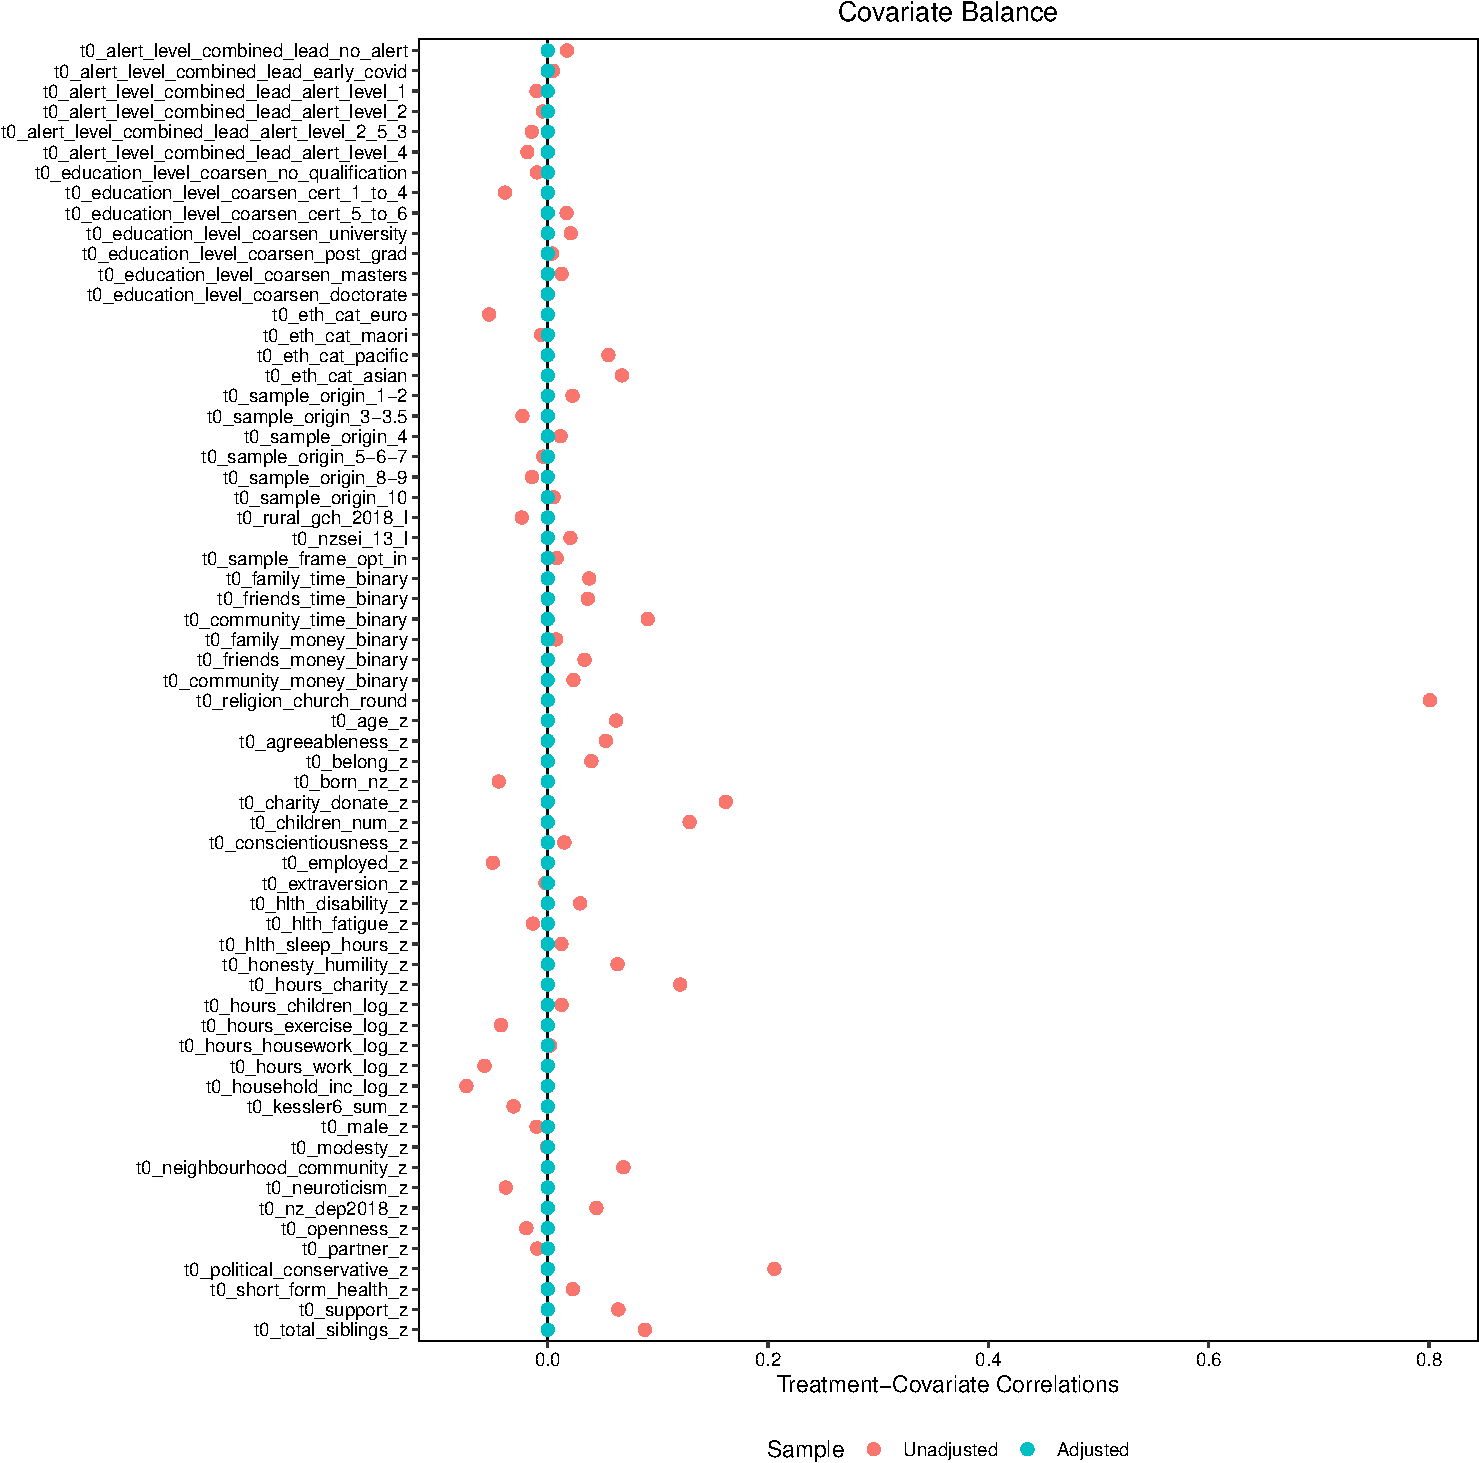
\includegraphics{test_files/figure-pdf/fig-match_1-1.pdf}

}

\caption{\label{fig-match_1}This figure shows the imbalance in
covariates on the treatment}

\end{figure}%

\subsection{Appendix D: Baseline and End of Study Outcome
Statistics}\label{appendix-outcomes}

\begin{longtable}[]{@{}
  >{\raggedright\arraybackslash}p{(\columnwidth - 4\tabcolsep) * \real{0.4474}}
  >{\raggedright\arraybackslash}p{(\columnwidth - 4\tabcolsep) * \real{0.2763}}
  >{\raggedright\arraybackslash}p{(\columnwidth - 4\tabcolsep) * \real{0.2763}}@{}}

\caption{\label{tbl-table-outcomes}Outcomes at baseline and
end-of-study}

\tabularnewline

\toprule\noalign{}
\begin{minipage}[b]{\linewidth}\raggedright
\textbf{Outcome Variables by Wave}
\end{minipage} & \begin{minipage}[b]{\linewidth}\raggedright
\textbf{2018}, N = 33,198
\end{minipage} & \begin{minipage}[b]{\linewidth}\raggedright
\textbf{2020}, N = 33,198
\end{minipage} \\
\midrule\noalign{}
\endhead
\bottomrule\noalign{}
\endlastfoot
\textbf{Annual Charity} & 150 (40, 500) & 200 (20, 600) \\
Unknown & 1,076 & 6,730 \\
\textbf{Community Gives Money Binary} & 135 (0.4\%) & 118 (0.4\%) \\
Unknown & 669 & 6,959 \\
\textbf{Community Gives Time Binary} & 1,702 (5.2\%) & 1,669 (6.4\%) \\
Unknown & 669 & 6,959 \\
\textbf{Family Gives Money Binary} & 1,782 (5.5\%) & 1,236 (4.7\%) \\
Unknown & 669 & 6,959 \\
\textbf{Family Gives Time Binary} & 9,539 (29\%) & 7,600 (29\%) \\
Unknown & 669 & 6,959 \\
\textbf{Friends Give Money Binary} & 372 (1.1\%) & 270 (1.0\%) \\
Unknown & 669 & 6,959 \\
\textbf{Friends Give Time} & 5,765 (18\%) & 4,855 (19\%) \\
Unknown & 669 & 6,959 \\
\textbf{Sense Neighbourhood Community} & NA & NA \\
1 & 1,976 (6.0\%) & 1,124 (4.2\%) \\
2 & 4,037 (12\%) & 2,703 (10\%) \\
3 & 4,796 (15\%) & 3,561 (13\%) \\
4 & 6,840 (21\%) & 5,809 (22\%) \\
5 & 7,088 (21\%) & 6,477 (24\%) \\
6 & 5,753 (17\%) & 5,060 (19\%) \\
7 & 2,550 (7.7\%) & 2,104 (7.8\%) \\
Unknown & 158 & 6,360 \\
\textbf{Social Belonging} & 5.33 (4.33, 6.00) & 5.33 (4.33, 6.00) \\
Unknown & 268 & 6,418 \\
\textbf{Social Support} & 6.33 (5.33, 7.00) & 6.33 (5.33, 7.00) \\
Unknown & 19 & 6,286 \\
\textbf{Volunteering Hours} & 0.00 (0.00, 1.00) & 0.00 (0.00, 1.00) \\
Unknown & 875 & 6,863 \\
\textbf{Volunteers Binary} & 9,443 (29\%) & 6,881 (26\%) \\
Unknown & 875 & 6,863 \\

\end{longtable}

Table~\ref{tbl-table-outcomes} presents baseline and end-of-study
descriptive statistics for the outcome variables.

\newpage{}

\subsection*{References}\label{references}
\addcontentsline{toc}{subsection}{References}

\phantomsection\label{refs}
\begin{CSLReferences}{1}{0}
\bibitem[\citeproctext]{ref-angrist2009mostly}
Angrist, Joshua D, and Jörn-Steffen Pischke. 2009. \emph{Mostly Harmless
Econometrics: An Empiricist's Companion}. Princeton university press.

\bibitem[\citeproctext]{ref-athey2019}
Athey, Susan, Julie Tibshirani, and Stefan Wager. 2019. {``Generalized
Random Forests.''} \emph{The Annals of Statistics} 47 (2): 1148--78.
\url{https://doi.org/10.1214/18-AOS1709}.

\bibitem[\citeproctext]{ref-athey2021}
Athey, Susan, and Stefan Wager. 2021. {``Policy Learning With
Observational Data.''} \emph{Econometrica} 89 (1): 133--61.
\url{https://doi.org/10.3982/ECTA15732}.

\bibitem[\citeproctext]{ref-atkinson2019}
Atkinson, J, C Salmond, and P Crampton. 2019. {``NZDep2018 Index of
Deprivation, User{'}s Manual.''} Wellington.

\bibitem[\citeproctext]{ref-bekkers2011literature}
Bekkers, René, and Pamala Wiepking. 2011. {``A Literature Review of
Empirical Studies of Philanthropy: Eight Mechanisms That Drive
Charitable Giving.''} \emph{Nonprofit and Voluntary Sector Quarterly} 40
(5): 924--73.

\bibitem[\citeproctext]{ref-brooks2004faith}
Brooks, Arthur C. 2004. {``Faith, Secularism, and Charity.''}
\emph{Faith \& Economics} 43 (Spring): 1--8.

\bibitem[\citeproctext]{ref-bulbulia2022}
Bulbulia, J. A. 2022. {``A Workflow for Causal Inference in
Cross-Cultural Psychology.''} \emph{Religion, Brain \& Behavior} 0 (0):
1--16. \url{https://doi.org/10.1080/2153599X.2022.2070245}.

\bibitem[\citeproctext]{ref-bulbulia2023}
---------. 2023. {``Causal Diagrams (Directed Acyclic Graphs): A
Practical Guide.''}

\bibitem[\citeproctext]{ref-Bulbulia_2015}
Bulbulia, J. A., J. H. Shaver, L. Greaves, R. Sosis, and C. G. Sibley.
2015. {``Religion and Parental Cooperation: An Empirical Test of Slone's
Sexual Signaling Model.''} In \emph{The Attraction of Religion: A Sexual
Selectionist Account}, edited by Slone J. D. amd Van Slyke J., 29--62.
Bloomsbury Press.

\bibitem[\citeproctext]{ref-bulbulia2012spreading}
Bulbulia, Joseph. 2012. {``Spreading Order: Religion, Cooperative Niche
Construction, and Risky Coordination Problems.''} \emph{Biology \&
Philosophy} 27: 1--27.

\bibitem[\citeproctext]{ref-bulbulia2024PRACTICAL}
---------. 2024. {``A Practical Guide to Causal Inference in Three-Wave
Panel Studies.''} \emph{PsyArXiv Preprints}, February.
\url{https://doi.org/10.31234/osf.io/uyg3d}.

\bibitem[\citeproctext]{ref-margot2024}
Bulbulia, Joseph A. 2024. \emph{Margot: MARGinal Observational
Treatment-Effects}. \url{https://doi.org/10.5281/zenodo.10907724}.

\bibitem[\citeproctext]{ref-bulbulia2023a}
Bulbulia, Joseph A, M Usman Afzali, Kumar Yogeeswaran, and Chris G
Sibley. 2023. {``Long-Term Causal Effects of Far-Right Terrorism in
{N}ew {Z}ealand.''} \emph{PNAS Nexus} 2 (8): pgad242.

\bibitem[\citeproctext]{ref-campbell2004}
Campbell, W Keith, Angelica M Bonacci, Jeremy Shelton, Julie J Exline,
and Brad J Bushman. 2004. {``Psychological Entitlement: Interpersonal
Consequences and Validation of a Self-Report Measure.''} \emph{Journal
of Personality Assessment} 83 (1): 29--45.

\bibitem[\citeproctext]{ref-chatton2020}
Chatton, Arthur, Florent Le Borgne, Clémence Leyrat, Florence
Gillaizeau, Chloé Rousseau, Laetitia Barbin, David Laplaud, Maxime
Léger, Bruno Giraudeau, and Yohann Foucher. 2020. {``G-Computation,
Propensity Score-Based Methods, and Targeted Maximum Likelihood
Estimator for Causal Inference with Different Covariates Sets: A
Comparative Simulation Study.''} \emph{Scientific Reports} 10 (1): 9219.
\url{https://doi.org/10.1038/s41598-020-65917-x}.

\bibitem[\citeproctext]{ref-xgboost2023}
Chen, Tianqi, Tong He, Michael Benesty, Vadim Khotilovich, Yuan Tang,
Hyunsu Cho, Kailong Chen, et al. 2023. \emph{Xgboost: Extreme Gradient
Boosting}. \url{https://CRAN.R-project.org/package=xgboost}.

\bibitem[\citeproctext]{ref-chen2020religious}
Chen, Ying, Eric S Kim, and Tyler J VanderWeele. 2020.
{``Religious-Service Attendance and Subsequent Health and Well-Being
Throughout Adulthood: Evidence from Three Prospective Cohorts.''}
\emph{International Journal of Epidemiology} 49 (6): 2030--40.

\bibitem[\citeproctext]{ref-cristofori2016neural}
Cristofori, Irene, Joseph Bulbulia, John H Shaver, Marc Wilson, Frank
Krueger, and Jordan Grafman. 2016. {``Neural Correlates of Mystical
Experience.''} \emph{Neuropsychologia} 80: 212--20.

\bibitem[\citeproctext]{ref-danaei2012}
Danaei, Goodarz, Mohammad Tavakkoli, and Miguel A. Hernán. 2012. {``Bias
in observational studies of prevalent users: lessons for comparative
effectiveness research from a meta-analysis of statins.''}
\emph{American Journal of Epidemiology} 175 (4): 250--62.
\url{https://doi.org/10.1093/aje/kwr301}.

\bibitem[\citeproctext]{ref-decoulanges1903}
De Coulanges, Fustel. 1903. \emph{La Cité Antique: Étude Sur Le Culte,
Le Droit, Les Institutions de La Grèce Et de Rome}. Hachette.

\bibitem[\citeproctext]{ref-duxedaz2021}
Díaz, Iván, Nicholas Williams, Katherine L. Hoffman, and Edward J.
Schenck. 2021. {``Non-Parametric Causal Effects Based on Longitudinal
Modified Treatment Policies.''} \emph{Journal of the American
Statistical Association}.
\url{https://doi.org/10.1080/01621459.2021.1955691}.

\bibitem[\citeproctext]{ref-diaz2023lmtp}
---------. 2023. {``Nonparametric Causal Effects Based on Longitudinal
Modified Treatment Policies.''} \emph{Journal of the American
Statistical Association} 118 (542): 846--57.
\url{https://doi.org/10.1080/01621459.2021.1955691}.

\bibitem[\citeproctext]{ref-diaz2021nonparametric}
Dı́az, Iván, Nima S Hejazi, Kara E Rudolph, and Mark J van Der Laan.
2021. {``Nonparametric Efficient Causal Mediation with Intermediate
Confounders.''} \emph{Biometrika} 108 (3): 627--41.

\bibitem[\citeproctext]{ref-Diaz2023}
Dı́az, Iván, Nicholas Williams, and Kara E. Rudolph. 2023. \emph{Journal
of Causal Inference} 11 (1): 20220077.
\url{https://doi.org/doi:10.1515/jci-2022-0077}.

\bibitem[\citeproctext]{ref-fahy2017}
Fahy, Katie M., Alan Lee, and Barry J. Milne. 2017b. \emph{New Zealand
Socio-Economic Index 2013}. Wellington, New Zealand: Statistics New
Zealand-Tatauranga Aotearoa.

\bibitem[\citeproctext]{ref-fahy2017a}
---------. 2017a. \emph{New Zealand Socio-Economic Index 2013}.
Wellington, New Zealand: Statistics New Zealand-Tatauranga Aotearoa.

\bibitem[\citeproctext]{ref-fraser_coding_2020}
Fraser, Gloria, Joseph Bulbulia, Lara M. Greaves, Marc S. Wilson, and
Chris G. Sibley. 2020. {``Coding Responses to an Open-Ended Gender
Measure in a {N}ew {Z}ealand National Sample.''} \emph{The Journal of
Sex Research} 57 (8): 979--86.
\url{https://doi.org/10.1080/00224499.2019.1687640}.

\bibitem[\citeproctext]{ref-haneuse2013estimation}
Haneuse, Sebastian, and Andrea Rotnitzky. 2013. {``Estimation of the
Effect of Interventions That Modify the Received Treatment.''}
\emph{Statistics in Medicine} 32 (30): 5260--77.

\bibitem[\citeproctext]{ref-hazlett2022understanding}
Hazlett, Chad, and Leonard Wainstein. 2022. {``Understanding, Choosing,
and Unifying Multilevel and Fixed Effect Approaches.''} \emph{Political
Analysis} 30 (1): 46--65.

\bibitem[\citeproctext]{ref-hernan2024WHATIF}
Hernan, M. A., and J. M. Robins. 2024. \emph{Causal Inference: What If?}
Chapman \& Hall/CRC Monographs on Statistics \& Applied Probab. Taylor
\& Francis.
\url{https://www.hsph.harvard.edu/miguel-hernan/causal-inference-book/}.

\bibitem[\citeproctext]{ref-hernan2024stating}
Hernán, Miguel A, and Sander Greenland. 2024. {``Why Stating Hypotheses
in Grant Applications Is Unnecessary.''} \emph{JAMA} 331 (4): 285--86.

\bibitem[\citeproctext]{ref-hernuxe1n2016}
Hernán, Miguel A, Brian C Sauer, Sonia Hernández-Díaz, Robert Platt, and
Ian Shrier. 2016. {``Specifying a Target Trial Prevents Immortal Time
Bias and Other Self-Inflicted Injuries in Observational Analyses.''}
\emph{Journal of Clinical Epidemiology} 79: 70--75.

\bibitem[\citeproctext]{ref-hoffman2023}
Hoffman, Katherine L., Diego Salazar-Barreto, Kara E. Rudolph, and Iván
Díaz. 2023. {``Introducing Longitudinal Modified Treatment Policies: A
Unified Framework for Studying Complex Exposures,''} April.
\url{https://doi.org/10.48550/arXiv.2304.09460}.

\bibitem[\citeproctext]{ref-hoffman2022}
Hoffman, Katherine L., Edward J. Schenck, Michael J. Satlin, William
Whalen, Di Pan, Nicholas Williams, and Iván Díaz. 2022. {``Comparison of
a Target Trial Emulation Framework Vs Cox Regression to Estimate the
Association of Corticosteroids with COVID-19 Mortality.''} \emph{JAMA
Network Open} 5 (10): e2234425.
\url{https://doi.org/10.1001/jamanetworkopen.2022.34425}.

\bibitem[\citeproctext]{ref-hoverd_religious_2010}
Hoverd, William James, and Chris G Sibley. 2010. {``Religious and
Denominational Diversity in New Zealand 2009.''} \emph{New Zealand
Sociology} 25 (2): 59--87.

\bibitem[\citeproctext]{ref-huitfeldt2019collapsibility}
Huitfeldt, Anders, Mats J Stensrud, and Etsuji Suzuki. 2019. {``On the
Collapsibility of Measures of Effect in the Counterfactual Causal
Framework.''} \emph{Emerging Themes in Epidemiology} 16: 1--5.

\bibitem[\citeproctext]{ref-johnson2022global}
Johnson, Byron R, and Tyler J VanderWeele. 2022. {``The Global
Flourishing Study: A New Era for the Study of Well-Being.''}
\emph{International Bulletin of Mission Research} 46 (2): 272--75.

\bibitem[\citeproctext]{ref-johnson2005}
Johnson, Dominic DP. 2005. {``God{'}s Punishment and Public Goods: A
Test of the Supernatural Punishment Hypothesis in 186 World Cultures.''}
\emph{Human Nature} 16: 410--46.

\bibitem[\citeproctext]{ref-johnson2015}
---------. 2015. {``Big Gods, Small Wonder: Supernatural Punishment
Strikes Back.''} \emph{Religion, Brain \& Behavior} 5 (4): 290--98.

\bibitem[\citeproctext]{ref-jost_end_2006-1}
Jost, John T. 2006. {``The End of the End of Ideology.''} \emph{American
Psychologist} 61 (7): 651--70.
\url{https://doi.org/10.1037/0003-066X.61.7.651}.

\bibitem[\citeproctext]{ref-kelly2024religiosity}
Kelly, John Michael, Stephanie R Kramer, and Azim F Shariff. 2024.
{``Religiosity Predicts Prosociality, Especially When Measured by
Self-Report: A Meta-Analysis of Almost 60 Years of Research.''}
\emph{Psychological Bulletin} 150 (3): 284--318.

\bibitem[\citeproctext]{ref-khanna1995charity}
Khanna, Jyoti, John Posnett, and Todd Sandler. 1995. {``Charity
Donations in the UK: New Evidence Based on Panel Data.''} \emph{Journal
of Public Economics} 56 (2): 257--72.

\bibitem[\citeproctext]{ref-kim2019mediators}
Kim, Eric S, and Tyler J VanderWeele. 2019. {``Mediators of the
Association Between Religious Service Attendance and Mortality.''}
\emph{American Journal of Epidemiology} 188 (1): 96--101.

\bibitem[\citeproctext]{ref-konvalinka2011synchronized}
Konvalinka, Ivana, Dimitris Xygalatas, Joseph Bulbulia, Uffe Schjoedt,
Else-Marie Jegindo, Sebastian Wallot, Guy Van Orden, and Andreas
Roepstorff. 2011. {``Synchronized Arousal Between Performers and Related
Spectators in a Fire-Walking Ritual.''} \emph{Proceedings of the
National Academy of Sciences} 108 (20): 8514--19.

\bibitem[\citeproctext]{ref-van2012targeted}
Laan, Mark J van der, and Susan Gruber. 2012. {``Targeted Minimum Loss
Based Estimation of Causal Effects of Multiple Time Point
Interventions.''} \emph{The International Journal of Biostatistics} 8
(1).

\bibitem[\citeproctext]{ref-van2014discussion}
Laan, Mark J van der, Alexander R Luedtke, and Iván Dı́az. 2014.
{``Discussion of Identification, Estimation and Approximation of Risk
Under Interventions That Depend on the Natural Value of Treatment Using
Observational Data, by {J}essica {Y}oung, {M}iguel {H}ern{á}n, and
{J}ames {R}obins.''} \emph{Epidemiologic Methods} 3 (1): 21--31.

\bibitem[\citeproctext]{ref-lang2015effects}
Lang, Martin, Jan Krátkỳ, John H Shaver, Danijela Jerotijević, and
Dimitris Xygalatas. 2015. {``Effects of Anxiety on Spontaneous
Ritualized Behavior.''} \emph{Current Biology} 25 (14): 1892--97.

\bibitem[\citeproctext]{ref-lash2020}
Lash, T. L., K. J. Rothman, T. J. VanderWeele, and S. Haneuse. 2020.
\emph{Modern Epidemiology}. Wolters Kluwer.
\url{https://books.google.co.nz/books?id=SiTSnQEACAAJ}.

\bibitem[\citeproctext]{ref-vanderweelechurchmortality}
Li, Shanshan, Meir J. Stampfer, David R. Williams, and Tyler J.
VanderWeele. 2016. {``{Association of Religious Service Attendance With
Mortality Among Women}.''} \emph{JAMA Internal Medicine} 176 (6):
777--85. \url{https://doi.org/10.1001/jamainternmed.2016.1615}.

\bibitem[\citeproctext]{ref-linden2020EVALUE}
Linden, Ariel, Maya B Mathur, and Tyler J VanderWeele. 2020.
{``Conducting Sensitivity Analysis for Unmeasured Confounding in
Observational Studies Using e-Values: The Evalue Package.''} \emph{The
Stata Journal} 20 (1): 162--75.

\bibitem[\citeproctext]{ref-major2023exploring}
Major-Smith, Daniel. 2023. {``Exploring Causality from Observational
Data: An Example Assessing Whether Religiosity Promotes Cooperation.''}
\emph{Evolutionary Human Sciences} 5: e22.

\bibitem[\citeproctext]{ref-mccullough2020kindness}
McCullough, Michael E. 2020. \emph{The Kindness of Strangers: How a
Selfish Ape Invented a New Moral Code}. Simon; Schuster.

\bibitem[\citeproctext]{ref-mccullough2016christian}
McCullough, Michael E, Paul Swartwout, John H Shaver, Evan C Carter, and
Richard Sosis. 2016. {``Christian Religious Badges Instill Trust in
Christian and Non-Christian Perceivers.''} \emph{Psychology of Religion
and Spirituality} 8 (2): 149.

\bibitem[\citeproctext]{ref-mcelreath2020}
McElreath, Richard. 2020. \emph{Statistical Rethinking: A {B}ayesian
Course with Examples in r and Stan}. CRC press.

\bibitem[\citeproctext]{ref-McLeod2020}
McLeod, John. 2020. {``The New Zealand Support Report: The Current State
and Significance of Giving in New Zealand and the Outlook for
Recipients.''} JBWere.
\url{https://www.jbwere.co.nz/media/1qudxw3q/jbwere-nz-support-report-digital.pdf}.

\bibitem[\citeproctext]{ref-monsma2007religion}
Monsma, Stephen V. 2007. {``Religion and Philanthropic Giving and
Volunteering: Building Blocks for Civic Responsibility.''}
\emph{Interdisciplinary Journal of Research on Religion} 3.

\bibitem[\citeproctext]{ref-montgomery2018}
Montgomery, Jacob M., Brendan Nyhan, and Michelle Torres. 2018. {``How
Conditioning on Posttreatment Variables Can Ruin Your Experiment and
What to Do about It.''} \emph{American Journal of Political Science} 62
(3): 760--75. \url{https://doi.org/10.1111/ajps.12357}.

\bibitem[\citeproctext]{ref-diaz2012population}
Muñoz, Iván Dı́az, and Mark Van Der Laan. 2012. {``Population
Intervention Causal Effects Based on Stochastic Interventions.''}
\emph{Biometrics} 68 (2): 541--49.

\bibitem[\citeproctext]{ref-neal2020introduction}
Neal, Brady. 2020. {``Introduction to Causal Inference from a Machine
Learning Perspective.''} \emph{Course Lecture Notes (Draft)}.
\url{https://www.bradyneal.com/Introduction_to_Causal_Inference-Dec17_2020-Neal.pdf}.

\bibitem[\citeproctext]{ref-norenzayan2016}
Norenzayan, Ara, Azim F. Shariff, Will M. Gervais, Aiyana K. Willard,
Rita A. McNamara, Edward Slingerland, and Joseph Henrich. 2016. {``The
Cultural Evolution of Prosocial Religions.''} \emph{Behavioral and Brain
Sciences} 39 (January): e1.
\url{https://doi.org/10.1017/S0140525X14001356}.

\bibitem[\citeproctext]{ref-ogburn2021}
Ogburn, Elizabeth L., and Ilya Shpitser. 2021. {``Causal Modelling: The
Two Cultures.''} \emph{Observational Studies} 7 (1): 179--83.
\url{https://doi.org/10.1353/obs.2021.0006}.

\bibitem[\citeproctext]{ref-pawlikowski2019religious}
Pawlikowski, Jakub, Piotr Białowolski, Dorota Węziak-Białowolska, and
Tyler J VanderWeele. 2019. {``Religious Service Attendance, Health
Behaviors and Well-Being---an Outcome-Wide Longitudinal Analysis.''}
\emph{European Journal of Public Health} 29 (6): 1177--83.

\bibitem[\citeproctext]{ref-pearl2009}
Pearl, Judea. 2009. {``Causal Inference in Statistics: An Overview.''}
\url{https://doi.org/10.1214/09-SS057}.

\bibitem[\citeproctext]{ref-polley2023}
Polley, Eric, Erin LeDell, Chris Kennedy, and Mark van der Laan. 2023.
\emph{SuperLearner: Super Learner Prediction}.
\url{https://CRAN.R-project.org/package=SuperLearner}.

\bibitem[\citeproctext]{ref-richardson2023nested}
Richardson, Thomas S, Robin J Evans, James M Robins, and Ilya Shpitser.
2023. {``Nested {M}arkov Properties for Acyclic Directed Mixed
Graphs.''} \emph{The Annals of Statistics} 51 (1): 334--61.

\bibitem[\citeproctext]{ref-richardson2013swigsprimer}
Richardson, Thomas S, and James M Robins. 2013. {``Single World
Intervention Graphs: A Primer.''} In \emph{Second UAI Workshop on Causal
Structure Learning, {B}ellevue, {W}ashington}. Citeseer.
\url{https://citeseerx.ist.psu.edu/document?repid=rep1&type=pdf&doi=07bbcb458109d2663acc0d098e8913892389a2a7}.

\bibitem[\citeproctext]{ref-richardson2023potential}
---------. 2023. {``Potential Outcome and Decision Theoretic Foundations
for Statistical Causality.''} \emph{Journal of Causal Inference} 11 (1):
20220012.

\bibitem[\citeproctext]{ref-robins1986}
Robins, James. 1986. {``A New Approach to Causal Inference in Mortality
Studies with a Sustained Exposure Period---Application to Control of the
Healthy Worker Survivor Effect.''} \emph{Mathematical Modelling} 7
(9-12): 1393--1512.

\bibitem[\citeproctext]{ref-robins1992}
Robins, James M, and Sander Greenland. 1992. {``Identifiability and
Exchangeability for Direct and Indirect Effects.''} \emph{Epidemiology}
3 (2): 143--55.

\bibitem[\citeproctext]{ref-robins2010alternative}
Robins, James M, and Thomas S Richardson. 2010. {``Alternative Graphical
Causal Models and the Identification of Direct Effects.''}
\emph{Causality and Psychopathology: Finding the Determinants of
Disorders and Their Cures} 84: 103--58.

\bibitem[\citeproctext]{ref-rubin2005}
Rubin, Donald B. 2005. {``Causal Inference Using Potential Outcomes:
Design, Modeling, Decisions.''} \emph{Journal of the American
Statistical Association} 100 (469): 322--31.
\url{https://www.jstor.org/stable/27590541}.

\bibitem[\citeproctext]{ref-schloss2011evolutionary}
Schloss, Jeffrey P, and Michael J Murray. 2011. {``Evolutionary Accounts
of Belief in Supernatural Punishment: A Critical Review.''}
\emph{Religion, Brain \& Behavior} 1 (1): 46--99.

\bibitem[\citeproctext]{ref-shaver2015evolution}
Shaver, John H. 2015. {``The Evolution of Stratification in Fijian
Ritual Participation.''} \emph{Religion, Brain \& Behavior} 5 (2):
101--17.

\bibitem[\citeproctext]{ref-shaver2020church}
Shaver, John H, Eleanor A Power, Benjamin G Purzycki, Joseph Watts,
Rebecca Sear, Mary K Shenk, Richard Sosis, and Joseph A Bulbulia. 2020.
{``Church Attendance and Alloparenting: An Analysis of Fertility, Social
Support and Child Development Among {E}nglish Mothers.''}
\emph{Philosophical Transactions of the Royal Society B} 375 (1805):
20190428.

\bibitem[\citeproctext]{ref-shiba2021using}
Shiba, Koichiro, and Takuya Kawahara. 2021. {``Using Propensity Scores
for Causal Inference: Pitfalls and Tips.''} \emph{Journal of
Epidemiology} 31 (8): 457--63.

\bibitem[\citeproctext]{ref-shpitser2022multivariate}
Shpitser, Ilya, Thomas S Richardson, and James M Robins. 2022.
{``Multivariate Counterfactual Systems and Causal Graphical Models.''}
In \emph{Probabilistic and Causal Inference: The Works of {J}udea
{P}earl}, 813--52.

\bibitem[\citeproctext]{ref-shpitser2016causal}
Shpitser, Ilya, and Eric Tchetgen Tchetgen. 2016. {``Causal Inference
with a Graphical Hierarchy of Interventions.''} \emph{Annals of
Statistics} 44 (6): 2433.

\bibitem[\citeproctext]{ref-sibley2012}
Sibley, C. G., and J. A. Bulbulia. 2012. {``Healing Those Who Need
Healing: How Religious Practice Affects Social Belonging.''}
\emph{Journal for the Cognitive Science of Religion} 1: 29--45.

\bibitem[\citeproctext]{ref-sibley2021}
Sibley, Chris G. 2021. {``Sampling Procedure and Sample Details for the
New Zealand Attitudes and Values Study.''}
\url{https://doi.org/10.31234/osf.io/wgqvy}.

\bibitem[\citeproctext]{ref-sibley2011}
Sibley, Chris G, Nils Luyten, Missy Purnomo, Annelise Mobberley, Liz W
Wootton, Matthew D Hammond, Nikhil Sengupta, et al. 2011. {``The
Mini-IPIP6: Validation and Extension of a Short Measure of the Big-Six
Factors of Personality in New Zealand.''} \emph{New Zealand Journal of
Psychology} 40 (3): 142--59.

\bibitem[\citeproctext]{ref-sosis2005does}
Sosis, Richard. 2005. {``Does Religion Promote Trust?: The Role of
Signaling, Reputation, and Punishment.''} \emph{Interdisciplinary
Journal of Research on Religion} 1.

\bibitem[\citeproctext]{ref-sosis2003cooperation}
Sosis, Richard, and Eric R Bressler. 2003. {``Cooperation and Commune
Longevity: A Test of the Costly Signaling Theory of Religion.''}
\emph{Cross-Cultural Research} 37 (2): 211--39.

\bibitem[\citeproctext]{ref-neyman1923}
Splawa-Neyman, Jerzy, Dorota M Dabrowska, and Terrence P Speed. 1990.
{``On the Application of Probability Theory to Agricultural Experiments.
Essay on Principles. Section 9.''} \emph{Statistical Science}, 465--72.

\bibitem[\citeproctext]{ref-swanson1967}
Swanson, Guy E. 1967. {``Religion and Regime: A Sociological Account of
the {R}eformation.''}

\bibitem[\citeproctext]{ref-vanbuuren2018}
Van Buuren, Stef. 2018. \emph{Flexible Imputation of Missing Data}. CRC
press.

\bibitem[\citeproctext]{ref-van2014targeted}
Van der Laan, Mark J. 2014. {``Targeted Estimation of Nuisance
Parameters to Obtain Valid Statistical Inference.''} \emph{The
International Journal of Biostatistics} 10 (1): 29--57.

\bibitem[\citeproctext]{ref-vanderlaan2011}
Van Der Laan, Mark J., and Sherri Rose. 2011. \emph{Targeted Learning:
Causal Inference for Observational and Experimental Data}. Springer
Series in Statistics. New York, NY: Springer.
\url{https://link.springer.com/10.1007/978-1-4419-9782-1}.

\bibitem[\citeproctext]{ref-vanderlaan2018}
---------. 2018. \emph{Targeted Learning in Data Science: Causal
Inference for Complex Longitudinal Studies}. Springer Series in
Statistics. Cham: Springer International Publishing.
\url{http://link.springer.com/10.1007/978-3-319-65304-4}.

\bibitem[\citeproctext]{ref-vantongeren2020}
Van Tongeren, Daryl R, C Nathan DeWall, Zhansheng Chen, Chris G Sibley,
and Joseph Bulbulia. 2020. {``Religious Residue: Cross-Cultural Evidence
That Religious Psychology and Behavior Persist Following
Deidentification.''} \emph{Journal of Personality and Social
Psychology}.

\bibitem[\citeproctext]{ref-vanderweele2015}
VanderWeele, Tyler J. 2015. \emph{Explanation in Causal Inference:
Methods for Mediation and Interaction}. Oxford University Press.

\bibitem[\citeproctext]{ref-vanderweele2017causaleffectsService}
---------. 2017. {``Causal Effects of Religious Service Attendance?''}
\emph{Social Psychiatry and Psychiatric Epidemiology} 52: 1331--36.

\bibitem[\citeproctext]{ref-vanderweele2019}
---------. 2019. {``Principles of Confounder Selection.''}
\emph{European Journal of Epidemiology} 34 (3): 211--19.

\bibitem[\citeproctext]{ref-vanderweele2021can}
---------. 2021a. {``Can Sophisticated Study Designs with Regression
Analyses of Observational Data Provide Causal Inferences?''} \emph{JAMA
Psychiatry} 78 (3): 244--46.

\bibitem[\citeproctext]{ref-vanderweele2021effectsReligiousServiceMetanalysis}
---------. 2021b. {``Effects of Religious Service Attendance and
Religious Importance on Depression: Examining the Meta-Analytic
Evidence.''} \emph{The International Journal for the Psychology of
Religion} 31 (1): 21--26.

\bibitem[\citeproctext]{ref-vanderweele2009}
VanderWeele, Tyler J. 2009. {``Concerning the Consistency Assumption in
Causal Inference.''} \emph{Epidemiology} 20 (6): 880.
\url{https://doi.org/10.1097/EDE.0b013e3181bd5638}.

\bibitem[\citeproctext]{ref-vanderweele2017}
VanderWeele, Tyler J., and Peng Ding. 2017. {``Sensitivity Analysis in
Observational Research: Introducing the e-Value.''} \emph{Annals of
Internal Medicine} 167 (4): 268--74.
\url{https://doi.org/10.7326/M16-2607}.

\bibitem[\citeproctext]{ref-vanderweele2013}
VanderWeele, Tyler J, and Miguel A Hernan. 2013. {``Causal Inference
Under Multiple Versions of Treatment.''} \emph{Journal of Causal
Inference} 1 (1): 1--20.

\bibitem[\citeproctext]{ref-vanderweele2012MEASUREMENT}
VanderWeele, Tyler J., and Miguel A. Hernán. 2012. {``Results on
Differential and Dependent Measurement Error of the Exposure and the
Outcome Using Signed Directed Acyclic Graphs.''} \emph{American Journal
of Epidemiology} 175 (12): 1303--10.
\url{https://doi.org/10.1093/aje/kwr458}.

\bibitem[\citeproctext]{ref-vanderweele2020}
VanderWeele, Tyler J, Maya B Mathur, and Ying Chen. 2020.
{``Outcome-Wide Longitudinal Designs for Causal Inference: A New
Template for Empirical Studies.''} \emph{Statistical Science} 35 (3):
437--66.

\bibitem[\citeproctext]{ref-verbrugge1997}
Verbrugge, Lois M. 1997. {``A Global Disability Indicator.''}
\emph{Journal of Aging Studies} 11 (4): 337--62.
\url{https://doi.org/10.1016/S0890-4065(97)90026-8}.

\bibitem[\citeproctext]{ref-watts2016}
Watts, J., Bulbulia J. A., R. D. Gray, and Q. D. Atkinson. 2016.
{``Clarity and Causality Needed in Claims about Big Gods''} 39: 41--42.
\url{https://doi.org/DOI:10.1017/S0140525X15000576}.

\bibitem[\citeproctext]{ref-watts2015}
Watts, Joseph, Simon J Greenhill, Quentin D Atkinson, Thomas E Currie,
Joseph Bulbulia, and Russell D Gray. 2015. \emph{Broad Supernatural
Punishment but Not Moralizing High Gods Precede the Evolution of
Political Complexity in {A}ustronesia}. \emph{Proceedings of the Royal
Society B: Biological Sciences}. Vol. 282. 1804. The Royal Society.

\bibitem[\citeproctext]{ref-westreich2010}
Westreich, Daniel, and Stephen R. Cole. 2010. {``Invited commentary:
positivity in practice.''} \emph{American Journal of Epidemiology} 171
(6). \url{https://doi.org/10.1093/aje/kwp436}.

\bibitem[\citeproctext]{ref-westreich2013}
Westreich, Daniel, and Sander Greenland. 2013. {``The Table 2 Fallacy:
Presenting and Interpreting Confounder and Modifier Coefficients.''}
\emph{American Journal of Epidemiology} 177 (4): 292--98.

\bibitem[\citeproctext]{ref-wheatley1971}
Wheatley, Paul. 1971. \emph{The Pivot of the Four Quarters : A
Preliminary Enquiry into the Origins and Character of the Ancient
Chinese City}. Edinburgh University Press.
\url{https://cir.nii.ac.jp/crid/1130000795717727104}.

\bibitem[\citeproctext]{ref-whitehouse2023}
Whitehouse, Harvey, Pieter Francois, Patrick E. Savage, Daniel Hoyer,
Kevin C. Feeney, Enrico Cioni, Rosalind Purcell, et al. 2023. {``Testing
the Big Gods Hypothesis with Global Historical Data: A Review and
Retake.''} \emph{Religion, Brain \& Behavior} 13 (2): 124--66.

\bibitem[\citeproctext]{ref-williams2021}
Williams, Nicholas T., and Iván Díaz. 2021. \emph{{l}mtp: Non-Parametric
Causal Effects of Feasible Interventions Based on Modified Treatment
Policies}. \url{https://doi.org/10.5281/zenodo.3874931}.

\bibitem[\citeproctext]{ref-woodyard2014doing}
Woodyard, Ann, and John Grable. 2014. {``Doing Good and Feeling Well:
Exploring the Relationship Between Charitable Activity and Perceived
Personal Wellness.''} \emph{VOLUNTAS: International Journal of Voluntary
and Nonprofit Organizations} 25: 905--28.

\bibitem[\citeproctext]{ref-Ranger2017}
Wright, Marvin N., and Andreas Ziegler. 2017. {``{ranger}: A Fast
Implementation of Random Forests for High Dimensional Data in {C++} and
{R}.''} \emph{Journal of Statistical Software} 77 (1): 1--17.
\url{https://doi.org/10.18637/jss.v077.i01}.

\bibitem[\citeproctext]{ref-young2014identification}
Young, Jessica G, Miguel A Hernán, and James M Robins. 2014.
{``Identification, Estimation and Approximation of Risk Under
Interventions That Depend on the Natural Value of Treatment Using
Observational Data.''} \emph{Epidemiologic Methods} 3 (1): 1--19.

\bibitem[\citeproctext]{ref-zhang2023shouldMultipleImputation}
Zhang, Jiaxin, S Ghazaleh Dashti, John B Carlin, Katherine J Lee, and
Margarita Moreno-Betancur. 2023. {``Should Multiple Imputation Be
Stratified by Exposure Group When Estimating Causal Effects via Outcome
Regression in Observational Studies?''} \emph{BMC Medical Research
Methodology} 23 (1): 42.

\end{CSLReferences}



\end{document}
